\noindent Die Laplace-Transformation wird zur Beschreibung zeitkontinuierlicher Signale verwendet. Sie eignet sich zur L\"{o}sung linearer Differentialgleichungen mit konstanten Koeffizienten und wird zur Interpretation von linearen, zeitinvarianten Systemen mit \"{U}bertragungsfunktionen eingesetzt. Die Interpretation der \"{U}bertragungsfunktionen f\"{u}hrt zu Aussagen wie Stabilit\"{a}t, Schwingungsneigung, Kausalit\"{a}t und Sprungf\"{a}higkeit von Systemen. Die z-Transformation ist f\"{u}r zeitdiskrete Anwendungen das Pendant zur Laplace-Transformation. Sie wird in diesem Kapitel eingef\"{u}hrt und ist eine wichtige Voraussetzung f\"{u}r die Beschreibung zeitdiskreter Systeme und den Entwurf zeitdiskreter Filter. \medskip

\noindent Nach der Definition werden einige Korrespondenzen \"{u}ber die Definitionsgleichung bestimmt, und es wird ein Zusammenhang zwischen der z-Transformation und der Laplace-Transformation hergestellt.\medskip

\noindent Die eher aufwendige Bestimmung von Korrespondenzen \"{u}ber die Definitionsgleichung kann vermieden werden, wenn die vorliegende Funktion mit Rechenregeln auf Funktionen mit bekannten Korrespondenzen zur\"{u}ckgef\"{u}hrt werden kann. Die dazu notwendigen Rechenregeln werden hergeleitet und der ihr Nutzen an Beispielen aufgezeigt. \medskip

\noindent Die bei technischen Anwendungen entstehenden z-Transformierten sind typischerweise gebrochen rationale Funktionen. Die R\"{u}cktransformation vom z-Bereich in den Zeitbereich kann grunds\"{a}tzlich \"{u}ber ein Umkehrintegral erfolgen. Da dieser Weg aufwendig ist und Kenntnisse in der Funktionentheorie voraussetzt, wird er in der Praxis umgangen. Stattdessen wird die z-Transformierte in Partialbr\"{u}che zerlegt, die mit Hilfe der angesprochenen Rechenregeln und einiger Korrespondenzen in den Zeitbereich transformiert werden k\"{o}nnen.\medskip

\noindent Die computerunterst\"{u}tzte Berechnung von z-Transformierten wird anhand des Programms MATLAB aufgezeigt. Nach der Zusammenstellung der f\"{u}r die analytische Berechnung wesentlichen Befehle werden einige Beispiele und Beweise mit Hilfe der \textit{Symbolic Math Toolbox} berechnet.

\subsection{Grundlagen der z-Transformation}

\subsubsection{Definitionsgleichung der z-Transformation}

\noindent Die z-Transformation ist das \"{A}quivalent zur Laplace-Transformation. Zur Herleitung der Definitionsgleichung wird deshalb von der Laplace-Transformation ausgegangen. Wie bei der Laplace-Transformation werden nur kausale Signale betrachtet. Nach den Darstellungen zur Signalabtastung wird ein ideal abgetastetes kausales Signal \"{u}ber die Multiplikation des kontinuierlichen Signals mit einer Abtastfunktion dargestellt: 

\begin{equation}\label{eq:fiveone}
x_{A} \left(t\right)=\sum _{k=0}^{\infty }x\left(k\cdot T_{A} \right)\cdot \delta \left(t-k\cdot T_{A} \right) 
\end{equation}

\noindent Bei x${}_{A}$(t) handelt es sich um ein kontinuierliches Signal. Deshalb kann die Laplace-Transformierte berechnet werden zu 

\begin{equation}\label{eq:fivetwo}
X_{A} \left(s\right)=L\left\{\sum _{k=0}^{\infty }x\left(k\cdot T_{A} \right)\cdot \delta \left(t-k\cdot T_{A} \right) \right\}
\end{equation}

\noindent Da die Laplace-Transformation eine lineare Operation ist und der Term x$_{A}$(k$\cdot$T$_{A}$) nicht von der Zeit t abh\"{a}ngt, kann die Laplace-Transformierte umgerechnet werden in 

\begin{equation}\label{eq:fivethree}
\begin{split}
L\left\{\sum _{k=0}^{\infty }x(k\cdot T_{A} )\cdot \delta (t-k\cdot T_{A} ) \right\}=\sum _{k=0}^{\infty }x\left(k\cdot T_{A} \right)\cdot L\left\{\delta \left(t-k\cdot T_{A} \right)\right\} & =\sum _{k=0}^{\infty }x\left(k\cdot T_{A} \right)\cdot e^{-k\cdot T_{A} \cdot s} \\ 
& =\sum _{k=0}^{\infty }x\left[k\right]\cdot \left(e^{T_{A} \cdot s} \right)^{-k}
\end{split}
\end{equation}

\noindent Dabei ist die Variable s eine komplexe Zahl mit Real- und Imagin\"{a}rteil. Durch die Substitution von 

\begin{equation}\label{eq:fivefour}
z=e^{T_{A} \cdot s}
\end{equation}

\noindent kann die Schreibweise vereinfacht werden zu

\begin{equation}\label{eq:fivefive}
X\left(z\right)=\sum _{k=0}^{\infty }x\left[k\right]\cdot z^{-k}  
\end{equation}

\noindent Diese Gleichung ist die Definitionsgleichung der z-Transformation f\"{u}r kausale Signale. \"{A}hnlich wie bei den vorangegangenen Transformationen wird f\"{u}r die z-Transformation die Schreibweise 

\begin{equation}\label{eq:fivesix}
Z\left\{x\left[k\right]\right\}=X\left(z\right)
\end{equation}

\noindent und f\"{u}r die inverse z-Transformation die Schreibweise

\begin{equation}\label{eq:fiveseven}
Z^{-1} \left\{X\left(z\right)\right\}=x\left[k\right]
\end{equation}

\noindent eingef\"{u}hrt. Alternativ kann das Hantel-Symbol verwendet werden.

\begin{equation}\label{eq:fiveeight}
x\left[k\right]\circ -\bullet X\left(z\right)
\end{equation}

\subsubsection{z-Transformation grundlegender Signale}

\noindent Wie bei der Laplace-Transformation werden zun\"{a}chst einige Korrespondenzen der z-Transformation direkt \"{u}ber die Definitionsgleichung der z-Transformation berechnet. Dabei ergibt sich die z-Transformierte eines Signals durch Auswertung von endlichen und unendlichen Reihen.\bigskip

{\fontfamily{phv}\selectfont
\noindent\textbf{Diskrete Impulsfolge}}\smallskip

\noindent Aus der Definition der diskreten Impulsfolge 

\begin{equation}\label{eq:fivenine}
x\left[k\right]=\delta \left[k\right]=\left\{\begin{array}{l} {1 \quad \text{für k } = {\rm \; 0}} \\ 
{{\rm 0}\quad \text{für ganzzahlige k }\ne {\rm \; 0}} \end{array}\right.
\end{equation}

\noindent ergibt sich die z-Transformierte durch Einsetzen in die Definitionsgleichung zu

\begin{equation}\label{eq:fiveten}
X\left(z\right)=\sum _{k=0}^{\infty }\delta \left[k\right]\cdot z^{-k}  =1\cdot z^{0} =1
\end{equation}

\noindent Ist der Impuls um k${}_{0}$ verschoben, \"{a}ndert sich die z-Transformierte zu

\begin{equation}\label{eq:fiveeleven}
X\left(z\right)=\sum _{k=0}^{\infty }\delta \left[k-k_{0} \right]\cdot z^{-k}  =1\cdot z^{-k_{0} } =z^{-k_{0} }
\end{equation}

\noindent Der Vergleich der z-Transformierten von Impuls und verschobenem Impuls ist ein erster Hinweis auf eine Verschiebungsregel.\bigskip

{\fontfamily{phv}\selectfont
\noindent\textbf{Diskrete Rechteckfolge}}\smallskip

\noindent F\"{u}r die Rechteckfolge mit der Definition 

\begin{equation}\label{eq:fivetwelve}
x\left[k\right]=\sigma \left[k\right]-\sigma \left[k-K\right]
\end{equation}

\noindent wird die Summe in der Definitionsgleichung der z-Transformation endlich. Es gilt

\begin{equation}\label{eq:fivethirteen}
X\left(z\right)=\sum _{k=0}^{\infty }\left(\sigma \left[k\right]-\sigma \left[k-K\right]\right)\cdot z^{-k}  =\sum _{k=0}^{K}z^{-k}
\end{equation}

\noindent Die Auswertung der endlichen Summe mit den Rechenregeln f\"{u}r endliche geometrische Reihen 

\begin{equation}\label{eq:fivefourteen}
\sum _{k=0}^{K-1}q^{k}  =\frac{1-q^{K} }{1-q}
\end{equation}

\noindent ergibt die z-Transformierte

\begin{equation}\label{eq:fivefifteen}
X\left(z\right)=\sum _{k=0}^{\infty }\left(\sigma \left[k\right]-\sigma \left[k-K\right]\right)\cdot z^{-k}  =\frac{1-z^{-K} }{1-z^{-1} } 
\end{equation}

{\fontfamily{phv}\selectfont
\noindent\textbf{Diskrete Sprungfolge}}\smallskip

\noindent Die z-Transformation der Sprungfolge mit der Definition

\begin{equation}\label{eq:fivesixteen}
x\left[k\right]=\sigma \left[k\right]=\left\{\begin{array}{l} 
{1\rm \qquad \text{ für ganzzahlige k} \ge {\rm \; 0}} \\ 
{\rm 0 \qquad \text{ für ganzzahlige k} <{\rm \; 0}} \end{array}\right. 
\end{equation}

\noindent errechnet sich direkt durch Einsetzen in die Definitionsgleichung zu

\begin{equation}\label{eq:fiveseventeen}
X\left(z\right)=\sum _{k=0}^{\infty }\sigma \left[k\right]\cdot z^{-k}  =\sum _{k=0}^{\infty }z^{-k}  =\sum _{k=0}^{\infty }\left(z^{-1} \right)^{k} 
\end{equation}

\noindent Die Berechnung der Reihe kann auf die unendliche geometrische Reihe zur\"{u}ckgef\"{u}hrt werden. Die geometrische Reihe ist definiert als:

\begin{equation}\label{eq:fiveeighteen}
1+q+q^{2} +...=\sum _{k=0}^{\infty }q^{k} 
\end{equation}

\noindent Die Konvergenz der Reihe ist von dem Betrag der Gr\"{o}{\ss}e q abh\"{a}ngig. F\"{u}r einen Betrag {\textbar}q{\textbar} $\mathrm{<}$ 1 konvergiert die Reihe und kann berechnet werden zu

\begin{equation}\label{eq:fivenineteen}
\sum _{k=0}^{\infty }q^{k}  =\frac{1}{1-q} 
\end{equation}

\noindent Die Summe aus Gleichung \eqref{eq:fiveseventeen} ist eine geometrische Reihe, die f\"{u}r {\textbar}z${}^{-1}${\textbar} $\mathrm{<}$ 1 konvergiert und dargestellt werden kann als

\begin{equation}\label{eq:fivetwenty}
X\left(z\right)=\sum _{k=0}^{\infty }\left(z^{-1} \right)^{k}  =\frac{1}{1-z^{-1} } =\frac{z}{z-1}
\end{equation}

\noindent Auch an diesem Beispiel wird eine Verschiebung um k${}_{0}$ untersucht. 

\begin{equation}\label{eq:fivetwentyone}
X\left(z\right)=\sum _{k=0}^{\infty }\sigma \left[k-k_{0} \right]\cdot z^{-k}  =\sum _{k=k_{0} }^{\infty }z^{-k}  =\sum _{k=0}^{\infty }z^{-(k+k_{0} )}  =z^{-k_{0} } \cdot \sum _{k=0}^{\infty }z^{-k}  =z^{-k_{0} } \cdot \frac{z}{z-1}
\end{equation}

\noindent Die Auswertung der Beispiele Impulsfolge und Sprungfolge legt die Vermutung nahe, dass die Verschiebung einer Folge um k${}_{0}$ nach rechts generell einer Multiplikation der urspr\"{u}nglichen z-Transformierten mit ${\mathrm{z}}^{\mathrm{-}{\mathrm{k}}_0}\ $entspricht.\bigskip

{\fontfamily{phv}\selectfont
\noindent\textbf{Diskrete Exponentialfolge}}\smallskip

\noindent Die diskrete Exponentialfolge ist definiert als 

\begin{equation}\label{eq:fivetwentytwo}
x\left[k\right]=\lambda _{0}^{k} \cdot \sigma \left[k\right]
\end{equation}

\noindent mit

\begin{equation}\label{eq:fivetwentythree}
\lambda _{0} =r_{0} \cdot e^{j\cdot \Omega _{0} }
\end{equation}

\noindent Analog zur Sprungfolge ergibt sich die z-Transformierte zu

\begin{equation}\label{eq:fivetwentyfour}
X\left(z\right)=\sum _{k=0}^{\infty }\sigma \left[k\right]\cdot \lambda _{0}^{k} \cdot z^{-k}  =\sum _{k=0}^{\infty }\lambda _{0}^{k} \cdot z^{-k}  =\sum _{k=0}^{\infty }\left(\frac{\lambda _{0} }{z} \right)^{k} 
\end{equation}

\noindent Diese Gleichung kann f\"{u}r die Berechnung der Korrespondenz f\"{u}r die diskrete Exponentialfolge verwendet werden. Ist der Betrag von {\textbar}$\lambda_{0}\cdot z{}^{-1}${\textbar} $\mathrm{<}$ 1, konvergiert die Summe, und es gilt:

\begin{equation}\label{eq:fivetwentyfive}
X\left(z\right)=\sum _{k=0}^{\infty }\left(\lambda _{0} \cdot z^{-1} \right)^{k}  =\frac{1}{1-\lambda _{0} \cdot z^{-1} } =\frac{z}{z-\lambda _{0} }
\end{equation}

\noindent Die bislang berechneten z-Transformierten werden \"{u}ber die Definitionsgleichung berechnet. Zur Vereinfachung der Berechnung werden in Abschnitt 5.2 einige Rechenregeln der z-Transformation hergeleitet. 

\subsubsection{Existenz der z-Transformierten}

\noindent Bei der Berechnung einer z-Transformierten wird eine unendliche Reihe ausgewertet. Die z-Transformierte existiert nur dann, wenn diese Reihe konvergiert. Bei der Berechnung der z-Transformierten m\"{u}ssen teilweise Bedingungen an die Variable z gestellt werden, um die Konvergenz der Reihe sicherzustellen. Das f\"{u}hrt zu der Frage, unter welchen Bedingungen die z-Transformierte X(z) mit der Definitionsgleichung

\begin{equation}\label{eq:fivetwentysix}
X\left(z\right)=\sum _{k=0}^{\infty }x\left[k\right]\cdot z^{-k}
\end{equation}

\noindent existiert. F\"{u}r beidseitig begrenzte Signale x[k] mit begrenzter Amplitude konvergiert die Summe in Gleichung \eqref{eq:fivetwentysix} immer. Zur Untersuchung der Konvergenz dieser unendlichen Reihe wird die bei nur einseitig begrenzten Folgen x[k] werden die Folgen mit Hilfe einer Exponentialfolge nach oben abgesch\"{a}tzt. 

\begin{equation}\label{eq:fivetwentyseven}
\left|x\left[k\right]\right|\le M\cdot r^{k}
\end{equation}

\noindent Konvergiert die resultierende geometrische Reihe, existiert auch ihre z-Transformierte X(z). Mit der Absch\"{a}tzung der Folge x[k] gilt f\"{u}r X(z)

\begin{equation}\label{eq:fivetwentyeight}
X\left(z\right)=\sum _{k=0}^{\infty }x\left[k\right]\cdot z^{-k}  \le \sum _{k=0}^{\infty }\left|x\left[k\right]\cdot z^{-k} \right| \le \sum _{k=0}^{\infty }M\cdot r^{k} \cdot \left|z^{-k} \right| =M\cdot \sum _{k=0}^{\infty }\left|\frac{r}{z} \right|^{k}
\end{equation}

\noindent Damit existiert die z-Transformierte, wenn f\"{u}r den Betrag der Basis gilt:

\begin{equation}\label{eq:fivetwentynine}
\left|\frac{r}{z} \right|<1
\end{equation}

\noindent Diese Bedingung erf\"{u}llen alle Werte der z-Ebene, die au{\ss}erhalb des Kreises mit dem Radius r liegen. Bild \ref{fig:KonvergenzbereichZEbene} zeigt den Konvergenzbereich in der komplexen z-Ebene.
\clearpage
\begin{figure}[H]
  \centerline{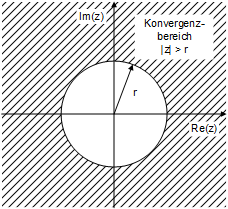
\includegraphics[width=0.4\textwidth]{Kapitel5/Bilder/image1.png}}
  \caption{Konvergenzbereich der z-Transformierten X(z) einer Folge x[k]}
  \label{fig:KonvergenzbereichZEbene}
\end{figure}

\noindent In praktischen Anwendungen k\"{o}nnen unendliche Signalfolgen mit einer Exponentialfolge nach oben abgesch\"{a}tzt werden, sodass die Konvergenz in den meisten F\"{a}llen gegeben ist. 

\subsubsection{Zusammenhang zwischen z-Transformation und Laplace-Transformation}

\noindent Mit Hilfe der Laplace-Transformation lassen sich einige Signaleigenschaften bestimmen. Um an diese Interpretationsm\"{o}glichkeiten anzukn\"{u}pfen, wird ein Zusammenhang zwischen der s-Ebene der Laplace-Transformation und der z-Ebene der z-Transformation hergestellt. Bei der Herleitung der z-Transformation wird die Substitution 

\begin{equation}\label{eq:fivethirty}
z=e^{T_{A} \cdot s} 
\end{equation}

\noindent verwendet. Mit dieser Substitution wird die komplexe s-Ebene in die komplexe z-Ebene abgebildet. Bild \ref{fig:VergleichSUndZEbene} zeigt die beiden Ebenen.

\begin{figure}[H]
  \centerline{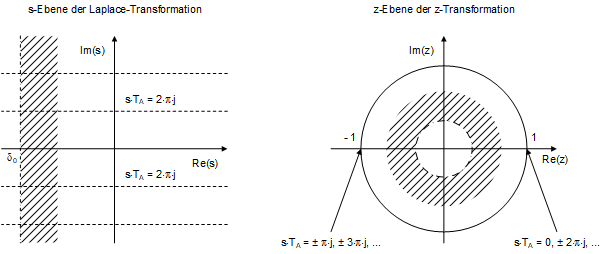
\includegraphics[width=1\textwidth]{Kapitel5/Bilder/image2.png}}
  \caption{Darstellung von Bereichen in der s-Ebene und deren transformierten Fl\"{a}chen in der z-Ebene}
  \label{fig:VergleichSUndZEbene}
\end{figure}

\noindent Die imagin\"{a}re Achse der s-Ebene s = j$\cdot\omega$ wird abgebildet in die Variable 

\begin{equation}\label{eq:fivethirtyone}
z=e^{j\cdot \omega \cdot T_{A} } 
\end{equation}

\noindent Das entspricht dem Einheitskreis, der f\"{u}r - $\infty$ $\mathrm{<}$ $\omega$ $\mathrm{<}$ $\infty$ periodisch in 2$\cdot\pi$ durchlaufen wird. Die imagin\"{a}re Achse der s-Ebene wird demnach auf den Einheitskreis der z-Ebene abgebildet. Bei der Abtastung von Signalen entsteht ein Spektrum, das periodisch in $\omega_{A}$ ist. Das Basisband reicht dabei von - $\omega_{A}$/2 bis +~$\omega_{A}$/2, so dass der Einheitskreis genau einmal durchlaufen wird. Alle periodischen Wiederholungen des Spektrums werden mit der z-Transformation auf dem Einheitskreis \"{u}bereinander abgebildet. Deshalb eignet sich die z-Transformation besonders f\"{u}r die Beschreibung abgetasteter Signale.

\noindent Eine Linie der s-Ebene mit konstantem Realteil $\delta_{0}$ wird auf einen Kreis abgebildet, der einen Radius 

\begin{equation}\label{eq:fivethirtytwo}
\left|z\right|=\left|e^{\left(\delta _{0} +j\cdot \omega \right)\cdot T_{A} } \right|=\left|e^{\delta _{0} \cdot T_{A} } \right|\cdot \left|e^{j\cdot \omega \cdot T_{A} } \right|=e^{\delta _{0} \cdot T_{A} } 
\end{equation}

\noindent aufweist. Mit negativem Realteil ergibt sich eine Lage innerhalb des Einheitskreises, mit positivem Realteil eine Lage um den Einheitskreis herum. Daraus folgt, dass die gesamte linke s-Halbebene in den Einheitskreis abgebildet wird, w\"{a}hrend die rechte s-Halbebene um den Einheitskreis herum abgebildet wird. Tabelle \ref{tab:fiveone} fasst korrespondierende Elemente der s- und z-Ebene zusammen.

\InsertBoxL{0}{
\includegraphics[scale=0.5]{Code.JPG}} 
\textcolor{white}{.}\newline
\noindent Im Online-Portal \textit{Systemtheorie Online} verdeutlicht die \textit{Applikation Signalabtastung und Signal-rekonstruktion} grafisch, welche Effekte durch Anti-Aliasing-Filter, reale Abtastung und reale Rekon-struktion entstehen.\newline   

\clearpage

\begin{table}[H]
\setlength{\arrayrulewidth}{.1em}
\caption{Tabellarische \"{U}bersicht \"{u}ber korrespondierende Elemente der s- und z-Ebene}
\setlength{\fboxsep}{0pt}%
\colorbox{lightgray}{%
\arrayrulecolor{white}%
\begin{tabular}{| c | c |}
\hline
\parbox[c][0.35in][c]{3.3in}{\smallskip\centering\textbf{\fontfamily{phv}\selectfont{s-Ebene}}} & \parbox[c][0.35in][c]{3.3in}{\smallskip\centering\textbf{\fontfamily{phv}\selectfont{z-Ebene}}}\\ \hline

\parbox[c][0.3in][c]{3.3in}{\centering{\fontfamily{phv}\selectfont{imaginäre Achse}}} & 
\parbox[c][0.3in][c]{3.3in}{\centering{\fontfamily{phv}\selectfont{Einheitskreis}}}\\ \hline

\parbox[c][0.3in][c]{3.3in}{\centering{\fontfamily{phv}\selectfont{linke komplexe Ebene}}} & 
\parbox[c][0.3in][c]{3.3in}{\centering{\fontfamily{phv}\selectfont{Inneres des Einheitskreises}}}\\ \hline

\parbox[c][0.3in][c]{3.3in}{\centering{\fontfamily{phv}\selectfont{rechte komplexe Ebene}}} & 
\parbox[c][0.3in][c]{3.3in}{\centering{\fontfamily{phv}\selectfont{Äußeres des Einheitskreises}}}\\ \hline

\parbox[c][0.3in][c]{3.3in}{\centering{\fontfamily{phv}\selectfont{Ursprung $s = 0$}}} & 
\parbox[c][0.3in][c]{3.3in}{\centering{$z = 1$}}\\ \hline

\parbox[c][0.4in][c]{3.3in}{\centering{\fontfamily{phv}\selectfont{halbe Abtastfrequenz j$\cdot\omega$ = j$\cdot\omega_{A}$/2 $\pm$ j$\cdot$k$\cdot\omega_{A}$}}} & 
\parbox[c][0.4in][c]{3.3in}{\centering{$z = - 1$}}\\ \hline

\end{tabular}%
}
\label{tab:fiveone}
\end{table}

\noindent Der Zusammenhang zwischen s- und z-Ebene wird bei der Diskussion der Signal- und Systemeigenschaften in den folgenden Abschnitten wieder aufgegriffen.

\subsubsection{Pollage und komplexe Exponential-Folge}

\noindent Im vorangegangenen Abschnitt wird die z-Transformierte der Exponentialfolge 

\begin{equation}\label{eq:fivethirtythree}
x\left[k\right]=\lambda _{0}^{k} \cdot \sigma \left[k\right]
\end{equation}

\noindent berechnet zu

\begin{equation}\label{eq:fivethirtyfour}
X\left(z\right)=\frac{z}{z-\lambda _{0} }
\end{equation}

\noindent Aus Gleichung \eqref{eq:fivethirtyfour} kann der zu der komplexen Exponentialfolge zugeh\"{o}rige Pol $\lambda_{0}$ in der komplexen z-Ebene abgelesen werden. Liegt der Pol auf der reellen Achse, handelt es sich um eine reelle Folge, die bei negativem Realteil alternierend ist. F\"{u}r einen Betrag von {\textbar}$\lambda_{0}${\textbar} $\mathrm{<}$ 1 ist die Folge konvergent, f\"{u}r {\textbar}$\lambda_{0}${\textbar} $\mathrm{>}$ 1 ist die Folge divergent und f\"{u}r {\textbar}$\lambda_{0}${\textbar} = 1 bleibt der Betrag der Folge konstant. Die Lage eines Poles in der z-Ebene kann damit einem Signalverhalten zugeordnet werden, das in Tabelle \ref{tab:fivetwo} skizziert wird.

\clearpage

\begin{table}[H]
\setlength{\arrayrulewidth}{.1em}
\caption{Tabellarische \"{U}bersicht \"{u}ber korrespondierende Elemente der s- und z-Ebene}
\setlength{\fboxsep}{0pt}%
\colorbox{lightgray}{%
\arrayrulecolor{white}%
\begin{tabular}{| c | c |}
\hline
\parbox[c][0.35in][c]{3.3in}{\smallskip\centering\textbf{\fontfamily{phv}\selectfont{Pollage X(z)}}} & \parbox[c][0.35in][c]{3.3in}{\smallskip\centering\textbf{\fontfamily{phv}\selectfont{Signalfolge x[k]}}}\\ \hline

\parbox[c][1.4in][c]{3.3in}{\centerline{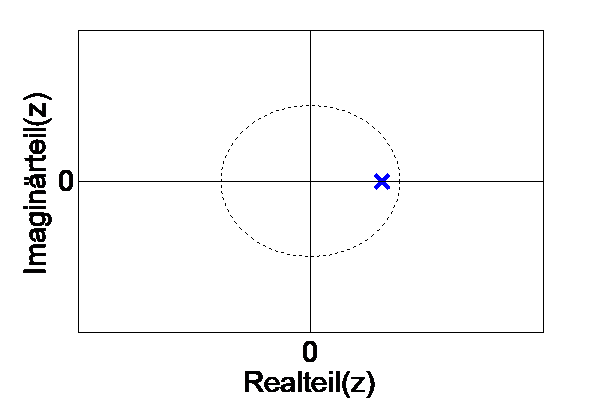
\includegraphics[width=0.3\textwidth]{Kapitel5/Table/image1.png}}} & 
\parbox[c][1.4in][c]{3.3in}{\centerline{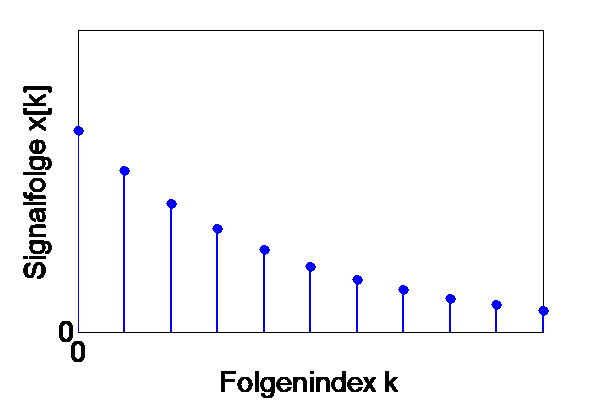
\includegraphics[width=0.3\textwidth]{Kapitel5/Table/image2.png}}}\\ \hline

\parbox[c][1.4in][c]{3.3in}{\centerline{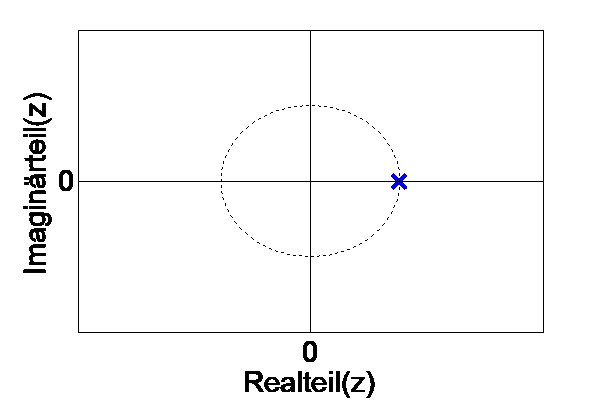
\includegraphics[width=0.3\textwidth]{Kapitel5/Table/image3.png}}} & 
\parbox[c][1.4in][c]{3.3in}{\centerline{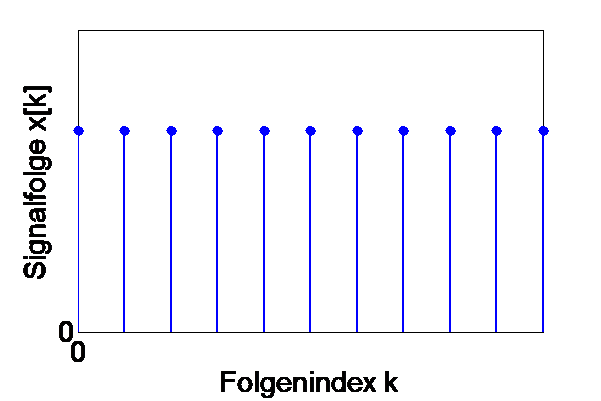
\includegraphics[width=0.3\textwidth]{Kapitel5/Table/image4.png}}}\\ \hline

\parbox[c][1.4in][c]{3.3in}{\centerline{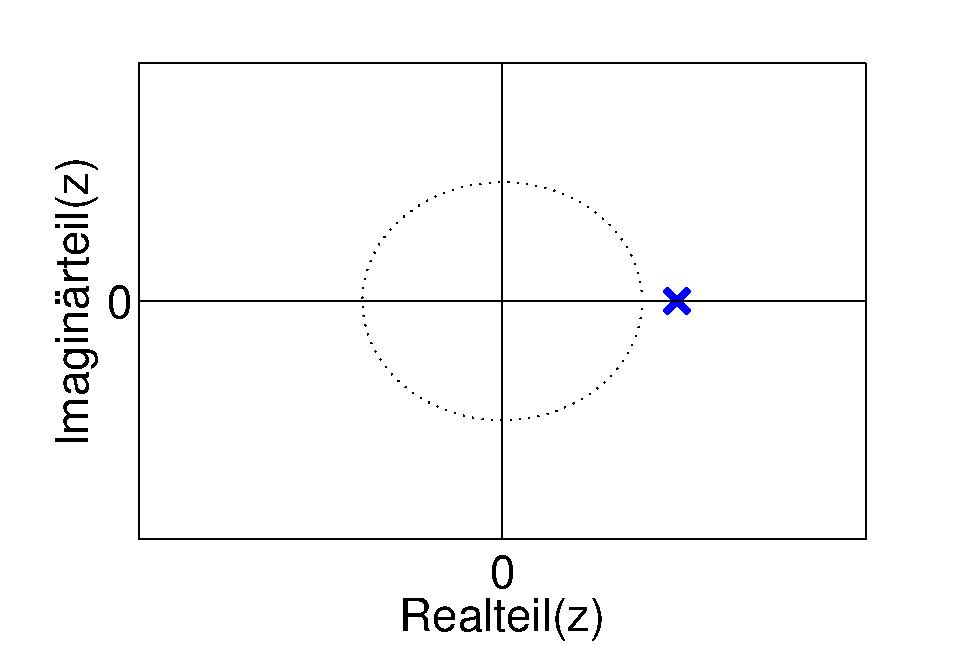
\includegraphics[width=0.3\textwidth]{Kapitel5/Table/image5.eps}}} & 
\parbox[c][1.4in][c]{3.3in}{\centerline{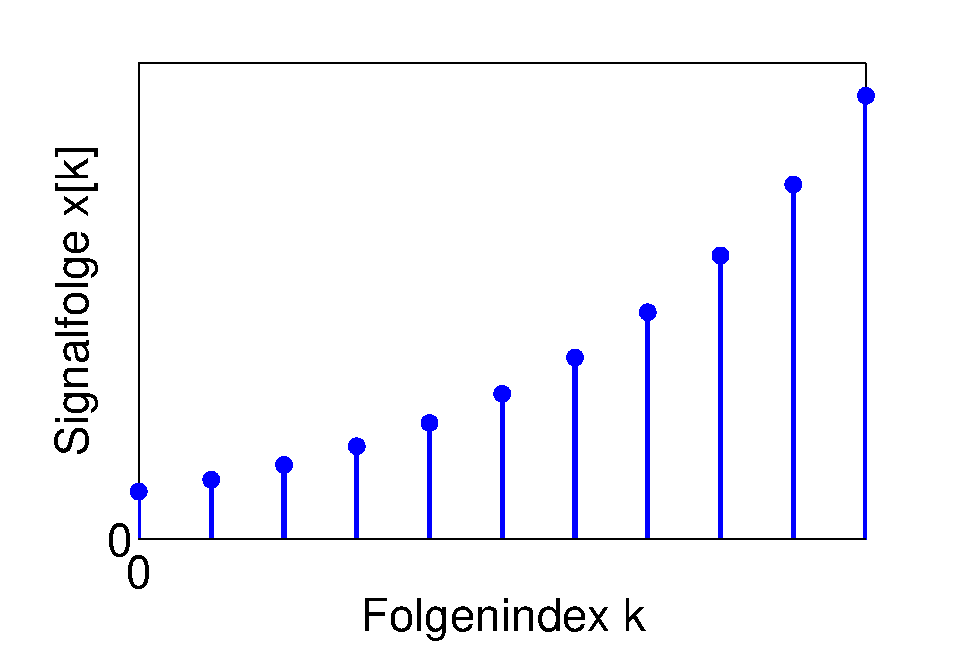
\includegraphics[width=0.3\textwidth]{Kapitel5/Table/image6.eps}}}\\ \hline

\parbox[c][1.4in][c]{3.3in}{\centerline{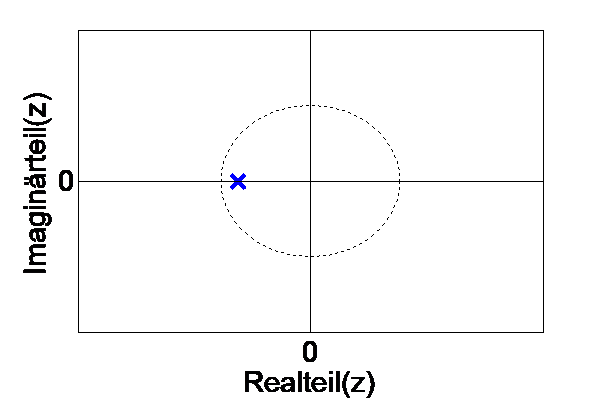
\includegraphics[width=0.3\textwidth]{Kapitel5/Table/image7.png}}} & 
\parbox[c][1.4in][c]{3.3in}{\centerline{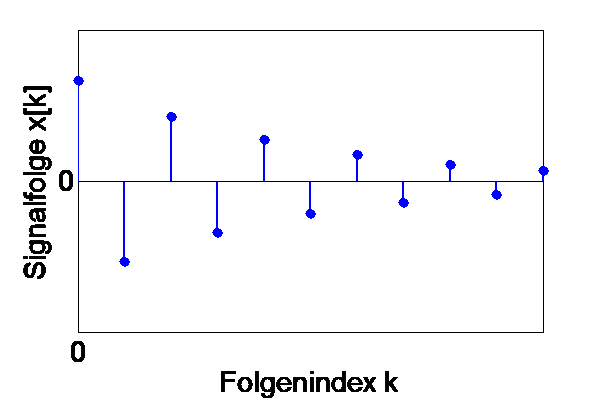
\includegraphics[width=0.3\textwidth]{Kapitel5/Table/image8.png}}}\\ \hline

\parbox[c][1.4in][c]{3.3in}{\centerline{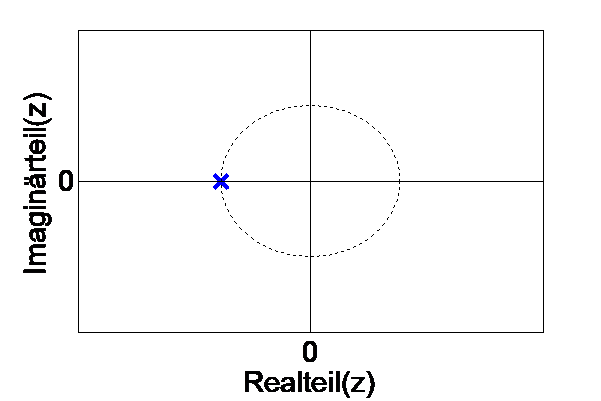
\includegraphics[width=0.3\textwidth]{Kapitel5/Table/image9.png}}} & 
\parbox[c][1.4in][c]{3.3in}{\centerline{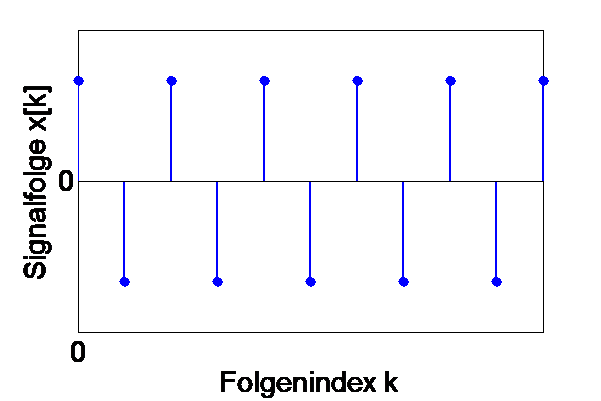
\includegraphics[width=0.3\textwidth]{Kapitel5/Table/image10.png}}}\\ \hline

\parbox[c][1.4in][c]{3.3in}{\centerline{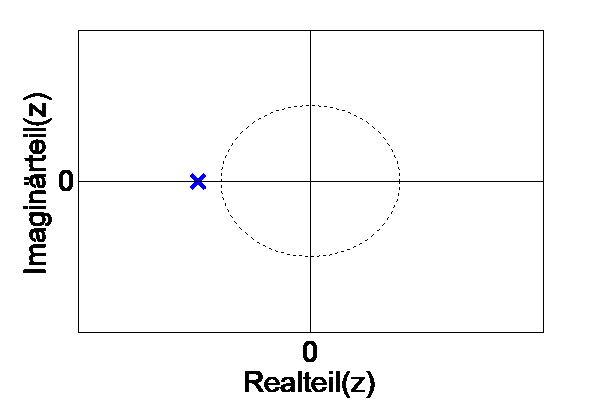
\includegraphics[width=0.3\textwidth]{Kapitel5/Table/image11.png}}} & 
\parbox[c][1.4in][c]{3.3in}{\centerline{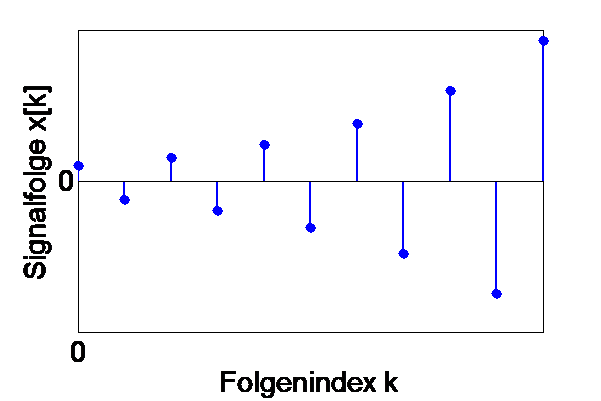
\includegraphics[width=0.3\textwidth]{Kapitel5/Table/image12.png}}}\\ \hline


\end{tabular}%
}
\label{tab:fivetwo}
\end{table}

\clearpage

\noindent Liegen z-Transformierte mit konjugiert komplexem Polpaare der Form

\begin{equation}\label{eq:fivethirtyfive}
X\left(z\right)=\frac{z}{z-r_{0} \cdot e^{j\cdot \Omega _{0} } } +\frac{z}{z-r_{0} \cdot e^{-j\cdot \Omega _{0} } } 
\end{equation}

\noindent vor, handelt es sich im Zeitbereich um Folgen der Form

\begin{equation}\label{eq:fivethirtysix}
x\left[k\right]=r_{0}^{k} \cdot \left(e^{j\cdot \Omega _{0} \cdot k} +e^{-j\cdot \Omega _{0} \cdot k} \right)\cdot \sigma \left[k\right]=2\cdot r_{0}^{k} \cdot \cos \left(\Omega _{0} \cdot k\right)\cdot \sigma \left[k\right]
\end{equation}

\noindent F\"{u}r einen Betrag von {\textbar}r${}_{0}${\textbar} $\mathrm{<}$ 1 ist die Folge konvergent, f\"{u}r {\textbar}r${}_{0}${\textbar} $\mathrm{>}$ 1 ist die Folge divergent und f\"{u}r {\textbar}r${}_{0}${\textbar} = 1 bleibt der Betrag der Folge konstant. Die Frequenz steigt mit wachsender Phase $\Omega_{0}$ des Pols, das Maximum wird erreicht f\"{u}r Pole mit einer Phase $\Omega_{0}$ = $\mathrm{\pm}$ $\pi$. Diese Interpretation entspricht bei entsprechender Umrechnung der Pole dem Zusammenhang zwischen der Pollage in der s-Ebene und der zugeh\"{o}rigen Zeitfunktion. Die Lage eines Poles in der z-Ebene kann damit einem Signalverhalten zugeordnet werden, das in Tabelle \ref{tab:fivethree} skizziert wird.

\begin{table}[H]
\setlength{\arrayrulewidth}{.1em}
\caption{Zusammenhang zwischen Pollage und Signalfolge bei konjugiert komplexen Polpaaren}
\setlength{\fboxsep}{0pt}%
\colorbox{lightgray}{%
\arrayrulecolor{white}%
\begin{tabular}{| c | c |}
\hline
\parbox[c][0.35in][c]{3.3in}{\smallskip\centering\textbf{\fontfamily{phv}\selectfont{Pollage X(z)}}} & \parbox[c][0.35in][c]{3.3in}{\smallskip\centering\textbf{\fontfamily{phv}\selectfont{Signalfolge x[k]}}}\\ \hline

\parbox[c][1.4in][c]{3.3in}{\centerline{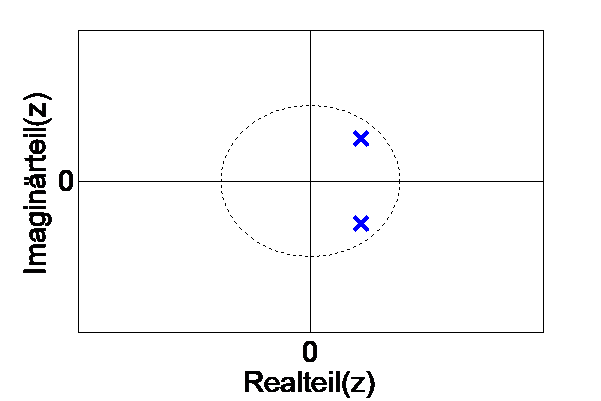
\includegraphics[width=0.3\textwidth]{Kapitel5/Table/image13.png}}} & 
\parbox[c][1.4in][c]{3.3in}{\centerline{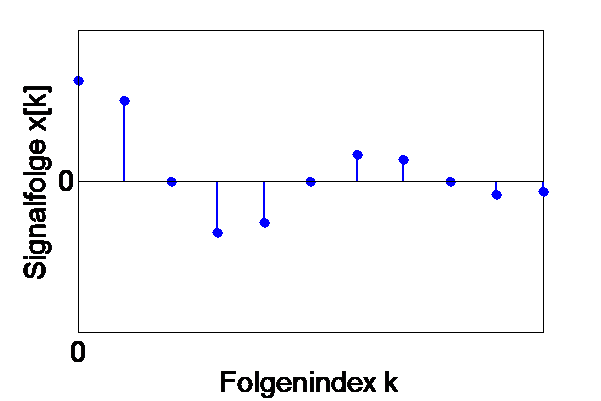
\includegraphics[width=0.3\textwidth]{Kapitel5/Table/image14.png}}}\\ \hline

\parbox[c][1.4in][c]{3.3in}{\centerline{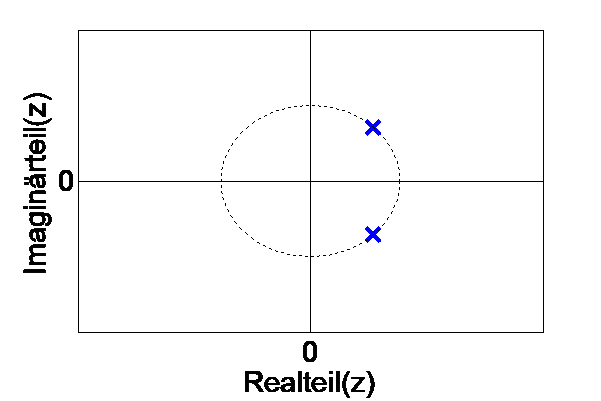
\includegraphics[width=0.3\textwidth]{Kapitel5/Table/image15.png}}} & 
\parbox[c][1.4in][c]{3.3in}{\centerline{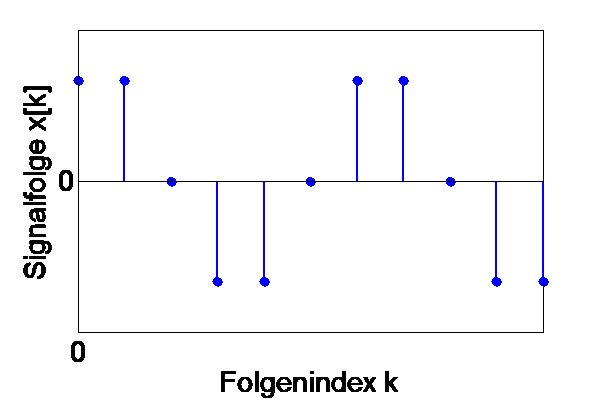
\includegraphics[width=0.3\textwidth]{Kapitel5/Table/image16.png}}}\\ \hline

\parbox[c][1.4in][c]{3.3in}{\centerline{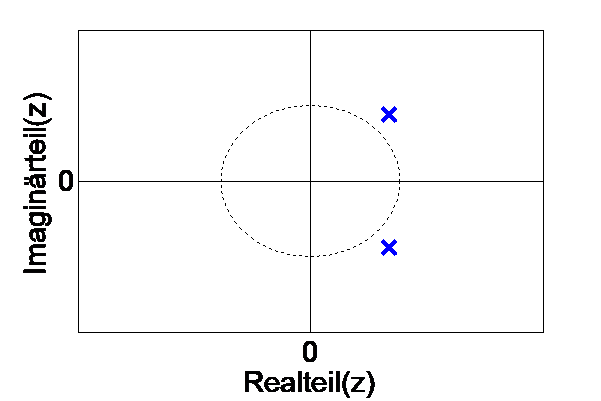
\includegraphics[width=0.3\textwidth]{Kapitel5/Table/image17.png}}} & 
\parbox[c][1.4in][c]{3.3in}{\centerline{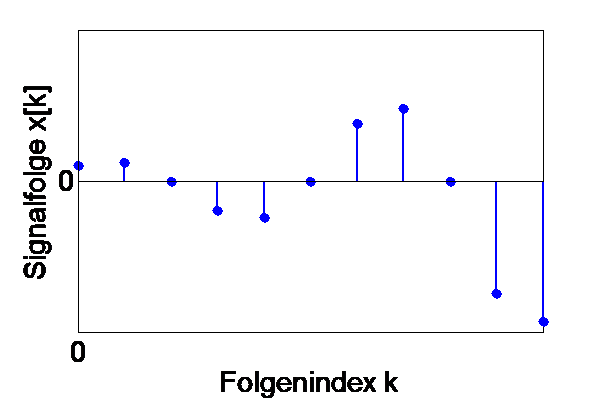
\includegraphics[width=0.3\textwidth]{Kapitel5/Table/image18.png}}}\\ \hline

\end{tabular}%
}
\label{tab:fivethree}
\end{table}

\InsertBoxL{0}{
\includegraphics[scale=0.5]{Code.JPG}} 
\textcolor{white}{.}\newline
\noindent Im Online-Portal \textit{Systemtheorie Online} verdeutlicht die \textit{Applikation Signalabtastung und Signal-rekonstruktion} grafisch, welche Effekte durch Anti-Aliasing-Filter, reale Abtastung und reale Rekon-struktion entstehen.\newline  

\clearpage

\subsection{Rechenregeln der z-Transformation}

\noindent Wie bei den bisher vorgestellten Transformationen besitzt die z-Transformation Rechenregeln, die das Rechnen und die Berechnung weiterer Korrespondenzen vereinfachen. Sie werden hergeleitet und ihr Nutzen an Beispielen verdeutlicht.

\subsubsection{Linearit\"{a}t}

\noindent Wie die Laplace- und die Fourier-Transformation ist auch die z-Transformation eine lineare Transformation. Durch Einsetzen in die Definitionsgleichung 

\begin{equation}\label{eq:fivethirtyseven}
Z\left\{\nu _{1} \cdot x_{1} \left[k\right]+\nu _{2} \cdot x_{2} \left[k\right]\right\}=\sum _{k=0}^{\infty }\left(\nu _{1} \cdot x_{1} \left[k\right]+\nu _{2} \cdot x_{2} \left[k\right]\right)\cdot z^{-k} 
\end{equation}

\noindent und durch Anwendung des Distributivgesetzes 

\begin{equation}\label{eq:fivethirtyeight}
\sum _{k=0}^{\infty }\left(\nu _{1} \cdot x_{1} \left[k\right]+\nu _{2} \cdot x_{2} \left[k\right]\right)\cdot z^{-k}  =\sum _{k=0}^{\infty }\nu _{1} \cdot x_{1} \left[k\right]\cdot z^{-k}  +\sum _{k=0}^{\infty }\nu _{2} \cdot x_{2} \left[k\right]\cdot z^{-k}  =\nu _{1} \cdot X_{1} \left(z\right)+\nu _{2} \cdot X_{2} \left(z\right)
\end{equation}

\noindent wird die Linearit\"{a}tseigenschaft bewiesen.\bigskip

\noindent
\colorbox{lightgray}{%
\arrayrulecolor{white}%
\renewcommand\arraystretch{0.6}%
\begin{tabular}{ wl{16.5cm} }
{\fontfamily{phv}\selectfont{Beispiel: Linearit\"{a}t} }
\end{tabular}%
}\medskip

\noindent Gesucht wird die z-Transformierte der Folge x[k]

\begin{equation}\label{eq:fivethirtynine}
x\left[k\right]=2\cdot \sigma \left[k\right]+5\cdot 3^{k} \cdot \sigma \left[k\right]
\end{equation}

\noindent Die z-Transformierten der Sprung- und Exponentialfolge sind bekannt. Damit ergibt sich X(z) zu

\begin{equation}\label{eq:fivefourty}
X\left(z\right)=2\cdot \frac{z}{z-1} +5\cdot \frac{z}{z-3}
\end{equation}

\subsubsection{Verschiebung der Folge nach rechts}

\noindent Bereits bei der Herleitung der verschobenen Impuls- und Sprungfolge wird die Verschiebungsregel der z-Transformation angedeutet. Die allgemeine Herleitung f\"{u}r eine Zeitverschiebung nach rechts ergibt sich f\"{u}r den Fall, dass x[k] eine kausale Folge ist, aus 

\begin{equation}\label{eq:fivefourtyone}
\begin{split}
Z\left\{x\left[k-k_{0} \right]\right\} & = \sum _{k=0}^{\infty }x\left[k-k_{0} \right]\cdot z^{-k}  =\sum _{k=k_{0} }^{\infty }x\left[k-k_{0} \right]\cdot z^{-k}  =\sum _{k=0}^{\infty }x[k]\cdot z^{-(k+k_{0} )}  =z^{-k_{0} } \cdot \sum _{k=0}^{\infty }x[k]\cdot z^{-k} \\
& = z^{- k_{0}}\cdot X(z)
\end{split}
\end{equation}

\noindent Diskrete Systeme lassen sich \"{u}ber Differenzengleichungen beschreiben. Aus diesem Grund ist die Verschiebungsregel von vergleichbarer Bedeutung wie die Differentiationsregel der Laplace-Transformation.

\clearpage

\noindent
\colorbox{lightgray}{%
\arrayrulecolor{white}%
\renewcommand\arraystretch{0.6}%
\begin{tabular}{ wl{16.5cm} }
{\fontfamily{phv}\selectfont{Beispiel: Verschiebung nach rechts}}
\end{tabular}%
}\medskip

\noindent Eine Rechteckfolge von 0 bis 4 kann im Zeitbereich dargestellt werden als

\begin{equation}\label{eq:fivefourtytwo}
x\left[k\right]=\sigma \left[k\right]-\sigma \left[k-5\right]
\end{equation}

\noindent Daraus ergibt sich mit der Verschiebungsregel die z-Transformierte zu

\begin{equation}\label{eq:fivefourtythree}
X\left(z\right)=\frac{z}{z-1} \cdot \left(1-z^{-5} \right)
\end{equation}

\subsubsection{Verschiebung der Folge nach links}

\noindent Die Regel zur Verschiebung nach links kann \"{a}hnlich hergeleitet werden wie die Regel zur Verschiebung nach rechts.

\begin{equation}\label{eq:fivefourtyfour}
Z\left\{x[k+k_{0} ]\right\}=\sum _{k=0}^{\infty }x[k+k_{0} ]\cdot z^{-k}  =z^{k_{0} } \cdot \sum _{k=0}^{\infty }x[k+k_{0} ]\cdot z^{-(k+k_{0} )}  =z^{k_{0} } \cdot \sum _{k=k_{0} }^{\infty }x[k]\cdot z^{-k}  
\end{equation}

\noindent Um die Summe bei k = 0 beginnen zu lassen, m\"{u}ssen einige Summanden addiert und wieder subtrahiert werden. Damit ergibt sich die Verschiebungsregel f\"{u}r eine Verschiebung nach links.

\begin{equation}\label{eq:fivefourtyfive}
\begin{split}
Z\left\{x\left[k+k_{0} \right]\right\} & = z^{k_{0} } \cdot \sum _{k=0}^{k_{0} -1}x\left[k\right]\cdot z^{-k}  +z^{k_{0} } \cdot \sum _{k=k_{0} }^{\infty }x\left[k\right]\cdot z^{-k}  -z^{k_{0} } \cdot \sum _{k=0}^{k_{0} -1}x\left[k\right]\cdot z^{-k} \\
& = z^{k_{0}} \cdot \sum _{k=0}^{\infty}x\left[k\right]\cdot z^{-k} - z^{k_{0}} \cdot \sum _{k=0}^{k_{0} -1}x\left[k\right]\cdot z^{-k} = z^{k_{0}}\cdot X(z) - z^{k_{0}}\cdot\sum _{k=0}^{k_{0} -1} x[k] \cdot z^{-k}
\end{split}
\end{equation}

\noindent Bei der Diskussion von Systemen im z-Bereich wird sich zeigen, dass sich diese Verschiebungsregel zur L\"{o}sung von Differenzengleichungen mit Anfangsbedingungen eignet. \bigskip

\noindent
\colorbox{lightgray}{%
\arrayrulecolor{white}%
\renewcommand\arraystretch{0.6}%
\begin{tabular}{ wl{16.5cm} }
{\fontfamily{phv}\selectfont{Beispiel: Verschiebung nach links}}
\end{tabular}%
}\medskip

\noindent Die Differenzengleichung 

\begin{equation}\label{eq:fivefourtysix}
x\left[k\right]-0.5\cdot x\left[k-1\right]=0 
\end{equation}

\noindent soll f\"{u}r den Anfangswert x[0] = 5 gel\"{o}st werden. Dazu wird die Differenzengleichung umgeformt zu

\begin{equation}\label{eq:fivefourtyseven}
x\left[k+1\right]-0.5\cdot x\left[k\right]=0
\end{equation}

\noindent und die Verschiebungsregel angewendet.

\begin{equation}\label{eq:fivefourtyeight}
z^{1} \cdot X\left(z\right)-x\left[0\right]\cdot z^{1} +0.5\cdot X\left(z\right)=0
\end{equation}

\noindent Aufl\"{o}sen nach X(z) f\"{u}hrt zu der z-Transformierten

\begin{equation}\label{eq:fivefourtynine}
X\left(z\right)=\frac{z\cdot x\left[0\right]}{z+0.5} =\frac{z\cdot 5}{z+0.5}
\end{equation}

\noindent Mit Hilfe der bereits diskutierten Rechenregeln kann die z-Transformierte in den Zeitbereich zur\"{u}cktransformiert werden.

\begin{equation}\label{eq:fivefifty}
x\left[k\right]=5\cdot \left(-0.5\right)^{k} \cdot \sigma \left[k\right]
\end{equation}

\subsubsection{Modulation}

\noindent Eine Modulation einer Folge x[k] mit der Exponentialfolge $\lambda^{k}$ l\"{a}sst sich im z-Bereich darstellen als

\begin{equation}\label{eq:fivefiftyone}
Z\left\{\lambda ^{k} \cdot x\left[k\right]\right\}=\sum _{k=0}^{\infty }\lambda ^{k} \cdot x\left[k\right]\cdot z^{-k}  =\sum _{k=0}^{\infty }x\left[k\right]\cdot \left(\frac{z}{\lambda } \right)^{-k}  =X\left(\frac{z}{\lambda } \right)
\end{equation}

\noindent
\colorbox{lightgray}{%
\arrayrulecolor{white}%
\renewcommand\arraystretch{0.6}%
\begin{tabular}{ wl{16.5cm} }
{\fontfamily{phv}\selectfont{Beispiel: Modulation}}
\end{tabular}%
}\medskip

\noindent Die Modulationsregel kann zum Nachweis der z-Transformierten der Exponentialfolge angewendet werden. Die z-Transformierte der Sprungfolge ist bekannt. Die Exponentialfolge ergibt sich aus

\begin{equation}\label{eq:fivefiftytwo}
x\left[k\right]=\lambda ^{k} \cdot \sigma \left[k\right]
\end{equation}

\noindent Nach der Modulationsregel ist damit die z-Transformierte der Exponentialfolge

\begin{equation}\label{eq:fivefiftythree}
X\left(z\right)=\left. \frac{z}{z-1} \right|_{z=\frac{z}{\lambda } } =\frac{\frac{z}{\lambda } }{\frac{z}{\lambda } -1} =\frac{z}{z-\lambda }
\end{equation}

\subsubsection{Lineare Gewichtung}

\noindent Die Eigenschaft der linearen Gewichtung ergibt sich durch Ableitung der z-Transformierten.

\begin{equation}\label{eq:fivefiftyfour}
\frac{dX}{dz} =\frac{d}{dz} \sum _{k=0}^{\infty }x\left[k\right]\cdot z^{-k}  =-k\cdot \sum _{k=0}^{\infty }x\left[k\right]\cdot z^{-k-1}  =-z^{-1} \cdot \sum _{k=0}^{\infty }k\cdot x\left[k\right]\cdot z^{-k}
\end{equation}

\noindent Multiplikation der Gleichung mit - z f\"{u}hrt zu der gesuchten Rechenregel der linearen Gewichtung. 

\begin{equation}\label{eq:fivefiftyfive}
Z\left\{k\cdot x\left[k\right]\right\}=\sum _{k=0}^{\infty }k\cdot x\left[k\right]\cdot z^{-k}  =-z\cdot \frac{dX}{dz}
\end{equation}

\clearpage

\noindent
\colorbox{lightgray}{%
\arrayrulecolor{white}%
\renewcommand\arraystretch{0.6}%
\begin{tabular}{ wl{16.5cm} }
{\fontfamily{phv}\selectfont{Beispiel: Gewichtung}}
\end{tabular}%
}\medskip

\noindent Die lineare Gewichtung wird dazu verwendet, die z-Transformierte der Rampenfolge 

\begin{equation}\label{eq:fivefiftysix}
x\left[k\right]=k\cdot \sigma \left[k\right]
\end{equation}

\noindent zu berechnen. Mit der Regel f\"{u}r die lineare Gewichtung und der z-Transformierten der Sprungfolge ergibt sich

\begin{equation}\label{eq:fivefiftyseven}
X\left(z\right)=-z\cdot \frac{d}{dz} \frac{z}{z-1} =-z\cdot \frac{z-1-z}{\left(z-1\right)^{2} } =\frac{z}{\left(z-1\right)^{2}} 
\end{equation}

\subsubsection{Differenz}

\noindent Die Differenz zweier aufeinanderfolgender Werte entspricht der Ableitung im zeitkontinuierlichen Bereich. Ihre z-Transformierte ergibt sich direkt aus dem Verschiebungssatz zu 

\begin{equation}\label{eq:fivefiftyeight}
Z\left\{x\left[k\right]-x\left[k-1\right]\right\}=\left(1-z^{-1} \right)\cdot X\left(z\right)=\frac{z-1}{z} \cdot X\left(z\right)
\end{equation}

\noindent
\colorbox{lightgray}{%
\arrayrulecolor{white}%
\renewcommand\arraystretch{0.6}%
\begin{tabular}{ wl{16.5cm} }
{\fontfamily{phv}\selectfont{Beispiel: Differenz}}
\end{tabular}%
}\medskip

\noindent Die Impulsfolge kann dargestellt werden als Differenz zweier Sprungfolgen:

\begin{equation}\label{eq:fivefiftynine}
\delta \left[k\right]=\sigma \left[k\right]-\sigma \left[k-1\right]
\end{equation}

\noindent Damit ergibt sich ihre z-Transformierte zu

\begin{equation}\label{eq:fivesixty}
X\left(z\right)=\frac{z-1}{z} \cdot \frac{z}{z-1} =1
\end{equation}

\noindent Das Ergebnis stimmt mit der Berechnung \"{u}ber die Definitionsgleichung \"{u}berein. 

\subsubsection{Summation}

\noindent Dem Integral f\"{u}r zeitkontinuierliche Funktionen entspricht bei Folgen die Summation. Zum Beweis der Summationsregel wird die Folge x[k] dargestellt als Differenz zweier Summen:

\begin{equation}\label{eq:fivesixtyone}
x\left[k\right]=\sum _{\kappa =0}^{k}x\left[\kappa \right]- \sum _{\kappa =0}^{k-1}x\left[\kappa \right]
\end{equation}

\noindent Die z-Transformation der Gleichung ergibt

\begin{equation}\label{eq:fivesixtytwo}
X\left(z\right)=\left(1-z^{-1} \right)\cdot Z\left(\sum _{\kappa =0}^{k}x\left[\kappa \right] \right)=\frac{z-1}{z} \cdot Z\left(\sum _{\kappa =0}^{k}x\left[\kappa \right] \right)
\end{equation}

\noindent Durch Umstellen ergibt sich die Summationsregel der z-Transformation

\begin{equation}\label{eq:fivesixtythree}
Z\left\{\sum _{\kappa =0}^{k}x\left[\kappa \right] \right\}=\frac{z}{z-1} \cdot X(z)
\end{equation}

\noindent
\colorbox{lightgray}{%
\arrayrulecolor{white}%
\renewcommand\arraystretch{0.6}%
\begin{tabular}{ wl{16.5cm} }
{\fontfamily{phv}\selectfont{Beispiel: Summation}}
\end{tabular}%
}\medskip

\noindent Die Sprungfolge kann als Summe \"{u}ber die Impulsfolge dargestellt werden.

\begin{equation}\label{eq:fivesixtyfour}
\sigma \left[k\right]=\sum _{\kappa =0}^{k}\delta \left[\kappa \right]
\end{equation}

\noindent Entsprechend ist der Zusammenhang zwischen den beiden z-Transformierten

\begin{equation}\label{eq:fivesixtyfive}
Z\left\{\sigma \left[k\right]\right\}=Z\left\{\sum _{\kappa =0}^{k}\delta \left[\kappa \right] \right\}=1\cdot \frac{z}{z-1} =\frac{z}{z-1}
\end{equation}

\noindent Auch die Rampenfolge l\"{a}sst sich als Summe \"{u}ber die Sprungfolge beschreiben. Dabei ist zu beachten, dass die Rampenfolge f\"{u}r k = 0 den Wert 0 besitzt. Damit ergibt sich f\"{u}r die Summe der Startwert k = 1 und die Summenformel der Rampenfolge lautet

\begin{equation}\label{eq:fivesixtysix}
x\left[k\right]=\sum _{\kappa =0}^{k}\sigma \left[\kappa -1\right]
\end{equation}

\noindent Mit der Summations- und Verschiebungsregel ergibt sich die z-Transformierte zu

\begin{equation}\label{eq:fivesixtyseven}
X\left(z\right)=\frac{z}{z-1} \cdot z^{-1} \cdot \frac{z}{z-1} =\frac{z}{\left(z-1\right)^{2} }
\end{equation}

\noindent Das Ergebnis stimmt mit der Berechnung \"{u}ber die lineare Gewichtung \"{u}berein. 

\subsubsection{Multiplikation}

\noindent Die Multiplikationsregel wird im folgenden Abschnitt mit Hilfe der R\"{u}cktransformation hergeleitet. Sie wird hier der Vollst\"{a}ndigkeit halber aufgef\"{u}hrt.

\begin{equation}\label{eq:fivesixtyeight}
Z\left\{x\left[k\right]\cdot y\left[k\right]\right\}=\frac{1}{2\cdot \pi \cdot j} \cdot \oint Y\left(\frac{z}{v} \right)\cdot X\left(v\right)\cdot v^{-1} {\rm \; }dv
\end{equation}

\subsubsection{Faltung}

\noindent Der Faltungssatz ist f\"{u}r die Berechnung von Systemantworten von gro{\ss}er Bedeutung und wird ausf\"{u}hrlich in Kapitel 8 behandelt. Die z-Transformierte der Faltung zweier Folgen ergibt sich durch Einsetzen in die Definitionsgleichung der z-Transformation zu

\begin{equation}\label{eq:fivesixtynine}
Z\left\{g\left[k\right]*x\left[k\right]\right\}=Z\left\{\sum _{\kappa =0}^{\infty }g\left[\kappa \right]\cdot x\left[k-\kappa \right] \right\}=\sum _{k=0}^{\infty }\sum _{\kappa =0}^{\infty }g\left[\kappa \right]\cdot x\left[k-\kappa \right]  \cdot z^{-k} 
\end{equation}

\noindent Vertauschen der Summationsreihenfolge und Substitution ergibt

\begin{equation}\label{eq:fiveseventy}
\begin{split}
\sum _{k=0}^{\infty }\sum _{\kappa =0}^{\infty }x\left[\kappa \right]\cdot g\left[k-\kappa \right]  \cdot z^{-k} &= \sum _{\kappa =0}^{\infty }\sum _{k=0}^{\infty }x\left[\kappa \right]\cdot g\left[k-\kappa \right]  \cdot z^{-k}\\
&= \sum _{k=0}^{\infty }x\left[\kappa \right]\cdot \sum _{k=0}^{\infty } g\left[k-\kappa \right] \cdot z^{-k} \cdot z^{\kappa} \cdot z^{-\kappa} \\
&= \sum _{k=0}^{\infty }x\left[\kappa \right]\cdot z^{-\kappa}\cdot \sum _{k=0}^{\infty } g\left[k-\kappa \right] \cdot z^{-k} \cdot z^{\kappa} \cdot z^{-(k-\kappa)}\\
&= \sum _{k=0}^{\infty }x\left[\kappa \right]\cdot z^{-\kappa}\cdot \sum _{k=0}^{\infty } g\left[n\right] \cdot z^{-n} = G(z) \cdot X(z)
\end{split}
\end{equation}

\noindent Diese Rechenregel wird bei der Diskussion zeitdiskreter Systeme im Bildbereich aufgegriffen.

\subsubsection{Anfangswertsatz}

\noindent Analog zu den Grenzwerts\"{a}tzen der Laplace-Transformation ergeben sich Anfangs- und Endwerts\"{a}tze der z-Transformation. Die Definitionsgleichung der z-Transformation lautet

\begin{equation}\label{eq:fiveseventyone}
X\left(z\right)=\sum _{k=0}^{\infty }x\left[k\right]\cdot z^{-k}  =x\left[0\right]+x\left[1\right]\cdot z^{-1} +x\left[2\right]\cdot z^{-2} +...
\end{equation}

\noindent Im Grenzfall z $\rightarrow$ $\infty$ werden alle Summanden, die einen Faktor z${}^{-k}$ mit k $\mathrm{>}$ 0 besitzen, zu null. \"{U}brig bleibt demnach der Ausdruck

\begin{equation}\label{eq:fiveseventytwo}
x\left[0\right]={\mathop{\lim }\limits_{z\to \infty }} X\left(z\right)
\end{equation}

\noindent Da bei der Herleitung des Anfangswertsatzes keine Einschr\"{a}nkung gemacht wird, kann diese Regel immer angewendet werden.\bigskip

\noindent
\colorbox{lightgray}{%
\arrayrulecolor{white}%
\renewcommand\arraystretch{0.6}%
\begin{tabular}{ wl{16.5cm} }
{\fontfamily{phv}\selectfont{Beispiel: Anfangswertsatz}}
\end{tabular}%
}\medskip

\noindent Die kausale Exponentialfolge besitzt die z-Transformierte 

\begin{equation}\label{eq:fiveseventythree}
X\left(z\right)=\frac{z}{z-\lambda _{0} }
\end{equation}

\noindent F\"{u}r den Grenz\"{u}bergang z $\rightarrow$ $\infty$ ergibt sich der Anfangswert zu

\begin{equation}\label{eq:fiveseventyfour}
{\mathop{\lim }\limits_{z\to \infty }} X\left(z\right)={\mathop{\lim }\limits_{z\to \infty }} \frac{z}{z-\lambda _{0} } ={\mathop{\lim }\limits_{z\to \infty }} \frac{1}{1-\frac{\lambda _{0} }{z} } =1
\end{equation}

\noindent Das Ergebnis stimmt mit dem Wert x[0] im Zeitbereich \"{u}berein. 

\clearpage

\subsubsection{Endwertsatz}

\noindent Zur Berechnung des Grenzwertes der Folge x[k] f\"{u}r k $\rightarrow$ $\infty$ wird vorausgesetzt, dass dieser Grenzwert existiert. Zur Herleitung des Endwertsatzes wird die z-Transformierte X(z) des Signals x[k] dargestellt als ein Produkt zweier z-Transformierter

\begin{equation}\label{eq:fiveseventyfive}
X\left(z\right)=\frac{z}{z-1} \cdot Y\left(z\right)
\end{equation}

\noindent Diese Gleichung kann mit der Faltungsregel in den Zeitbereich transformiert werden.

\begin{equation}\label{eq:fiveseventysix}
x\left[k\right]=\sum _{\kappa =0}^{\infty }y\left[n\right]\cdot \sigma \left[k-\kappa \right] =\sum _{\kappa =0}^{k}y\left[\kappa \right]
\end{equation}

\noindent F\"{u}r den Grenzwert k $\rightarrow$ $\infty$ kann die Summe dargestellt werden als

\begin{equation}\label{eq:fiveseventyseven}
{\mathop{\lim }\limits_{k\to \infty }} x\left[k\right]=\sum _{\kappa =0}^{\infty }y\left[\kappa \right] =\sum _{\kappa =0}^{\infty }y\left[\kappa \right] \cdot 1^{-\kappa } =Y\left(1\right)={\mathop{\lim }\limits_{z\to 1}} \frac{z-1}{z} \cdot X\left(z\right)={\mathop{\lim }\limits_{z\to 1}} \left(z-1\right)\cdot X\left(z\right)
\end{equation}

\noindent Mit der Definitionsgleichung der z-Transformation 

\begin{equation}\label{eq:fiveseventyeight}
Y\left(z\right)=\sum _{k=0}^{\infty }y\left[k\right]\cdot z^{-k}
\end{equation}

\noindent ergibt sich f\"{u}r z = 1 der Endwertsatz der z-Transformation

\begin{equation}\label{eq:fiveseventynine}
{\mathop{\lim }\limits_{k\to \infty }} x\left[k\right]=\sum _{\kappa =0}^{\infty }h\left[\kappa \right] \cdot 1^{-\kappa } =H\left(1\right)={\mathop{\lim }\limits_{z\to 1}} \frac{z-1}{z} \cdot X\left(z\right)={\mathop{\lim }\limits_{z\to 1}} \left(z-1\right)\cdot X\left(z\right)
\end{equation}

\noindent
\colorbox{lightgray}{%
\arrayrulecolor{white}%
\renewcommand\arraystretch{0.6}%
\begin{tabular}{ wl{16.5cm} }
{\fontfamily{phv}\selectfont{Beispiel: Endwertsatz}}
\end{tabular}%
}\medskip

\noindent Die kausale Exponentialfolge besitzt die z-Transformierte

\begin{equation}\label{eq:fiveeighty}
X\left(z\right)=\frac{z}{z-\lambda _{0} } 
\end{equation}

\noindent Mit dem Grenz\"{u}bergang z $\rightarrow$ 1 des Ausdrucks

\begin{equation}\label{eq:fiveeightyone}
{\mathop{\lim }\limits_{z\to 1}} \left(z-1\right)\cdot \frac{z}{z-\lambda _{0} } =0
\end{equation}

\noindent ergibt sich der Endwert von x[k] f\"{u}r k $\rightarrow$ $\infty$ zu null. Das Ergebnis stimmt mit dem Grenzwert im Zeitbereich \"{u}berein, wenn die Basis $\lambda_{0}$ einen Betrag {\textbar}$\lambda_{0}${\textbar} $\mathrm{<}$ 1 aufweist, also wenn ein Grenzwert existiert. 

\clearpage

\subsubsection{Zusammenfassung der Rechenregeln zur z-Transformation}

\noindent Zur besseren \"{U}bersicht stellt Tabelle \ref{tab:fivefour} die wesentlichen Eigenschaften der z-Transformation noch einmal zusammen.


\begin{table}[H]
\setlength{\arrayrulewidth}{.1em}
\caption{Rechenregeln der z-Transformation}
\setlength{\fboxsep}{0pt}%
\colorbox{lightgray}{%
\arrayrulecolor{white}%
\begin{tabular}{| c | c | c |}
\hline
\parbox[c][0.3in][c]{1.9in}{\smallskip\centering\textbf{\fontfamily{phv}\selectfont{Regel}}} & \parbox[c][0.3in][c]{2.2in}{\smallskip\centering\textbf{\fontfamily{phv}\selectfont{Funktion x(t)}}} &
\parbox[c][0.3in][c]{2.2in}{\smallskip\centering\textbf{\fontfamily{phv}\selectfont{Laplace-Transformierte X(s)}}}\\ \hline


\parbox[c][0.5in][c]{1.9in}{\centering{\fontfamily{phv}\selectfont{Linearität}}} & 
\parbox[c][0.5in][c]{2.2in}{\centering{$\nu _{1} \cdot x_{1} \left(t\right)+\nu _{2} \cdot x_{2} \left(t\right)$}} &
\parbox[c][0.5in][c]{2.2in}{\centering{$\nu _{1} \cdot X_{1} \left(s\right)+\nu _{2} \cdot X_{2} \left(s\right)$}}\\
\hline

\parbox[c][0.5in][c]{1.9in}{\centering{\fontfamily{phv}\selectfont{Zeitverschiebung nach rechts}}} & 
\parbox[c][0.5in][c]{2.2in}{\centering{$x\left[k-k_{0} \right]{\rm \; }$für${\rm \; }k_{0} >0$}} &
\parbox[c][0.5in][c]{2.2in}{\centering{$z^{-k_{0} } \cdot X\left(z\right)$}}\\
\hline

\parbox[c][0.5in][c]{1.9in}{\centering{\fontfamily{phv}\selectfont{Zeitverschiebung nach links}}} & 
\parbox[c][0.5in][c]{2.2in}{\centering{$x[k+k_{0} ]{\rm \; }$für${\rm \; }k_{0} >0$}} &
\parbox[c][0.5in][c]{2.2in}{\centering{$z^{k_{0} } \cdot X\left(z\right)-z^{k_{0} } \cdot \sum _{n=0}^{k_{0} -1}x\left[n\right]\cdot z^{-n}  $}}\\
\hline

\parbox[c][0.5in][c]{1.9in}{\centering{\fontfamily{phv}\selectfont{Modulation}}} & 
\parbox[c][0.5in][c]{2.2in}{\centering{$\lambda ^{k} \cdot x\left[k\right]$}} &
\parbox[c][0.5in][c]{2.2in}{\centering{$X\left(\frac{z}{\lambda } \right)$}}\\
\hline

\parbox[c][0.5in][c]{1.9in}{\centering{\fontfamily{phv}\selectfont{lineare Gewichtung}}} & 
\parbox[c][0.5in][c]{2.2in}{\centering{$k\cdot x\left[k\right]$}} &
\parbox[c][0.5in][c]{2.2in}{\centering{$-z\cdot \frac{d}{dz} \cdot X\left(z\right)$}}\\
\hline

\parbox[c][0.5in][c]{1.9in}{\centering{\fontfamily{phv}\selectfont{Differenz}}} & 
\parbox[c][0.5in][c]{2.2in}{\centering{$x\left[k\right]-x\left[k-1\right]$}} &
\parbox[c][0.5in][c]{2.2in}{\centering{$\frac{z-1}{z} \cdot X\left(z\right)$}}\\
\hline

\parbox[c][0.5in][c]{1.9in}{\centering{\fontfamily{phv}\selectfont{Summation}}} & 
\parbox[c][0.5in][c]{2.2in}{\centering{$\sum _{\kappa =0}^{k}x\left[\kappa \right] $ }} &
\parbox[c][0.5in][c]{2.2in}{\centering{$\frac{z}{z-1} \cdot X\left(z\right)$}}\\
\hline

\parbox[c][0.5in][c]{1.9in}{\centering{\fontfamily{phv}\selectfont{Multiplikation}}} & 
\parbox[c][0.5in][c]{2.2in}{\centering{$x_{1} \left[k\right]\cdot x_{2} \left[k\right]$}} &
\parbox[c][0.5in][c]{2.2in}{\centering{$\frac{1}{2\cdot \pi \cdot j} \cdot \oint X_{1} \left(\frac{z}{v} \right)\cdot X_{2} \left(v\right)\cdot v^{-1} {\rm \; }dv $}}\\
\hline

\parbox[c][0.5in][c]{1.9in}{\centering{\fontfamily{phv}\selectfont{Faltung}}} & 
\parbox[c][0.5in][c]{2.2in}{\centering{$g\left[k\right]*x\left[k\right]$ }} &
\parbox[c][0.5in][c]{2.2in}{\centering{$G\left(z\right)\cdot X\left(z\right)$}}\\
\hline

\parbox[c][0.5in][c]{1.9in}{\centering{\fontfamily{phv}\selectfont{Anfangswert}}} & 
\parbox[c][0.5in][c]{2.2in}{\centering{$x\left[0\right]$}} &
\parbox[c][0.5in][c]{2.2in}{\centering{${\mathop{\lim }\limits_{z\to \infty }} X\left(z\right)$}}\\
\hline

\parbox[c][0.5in][c]{1.9in}{\centering{\fontfamily{phv}\selectfont{Endwert}}} & 
\parbox[c][0.5in][c]{2.2in}{\centering{${\mathop{\lim }\limits_{k\to \infty}} x\left[k\right]$}} &
\parbox[c][0.5in][c]{2.2in}{\centering{${\mathop{\lim }\limits_{z\to 1}} \left(\left(z-1\right)\cdot X\left(z\right)\right)$}}\\
\hline
\end{tabular}%
}
\label{tab:fivefour}
\end{table}

\clearpage

\subsubsection{Korrespondenzen der z-Transformation}

\noindent Die Rechenregeln zur z-Transformation erlauben die Berechnung weiterer Korrespondenzen. Tabelle \ref{tab:fivefive} stellt wichtige Korrespondenzen der z-Transformation zusammen.

\begin{table}[H]
\setlength{\arrayrulewidth}{.1em}
\caption{Korrespondenzen der z-Transformation 1/2}
\setlength{\fboxsep}{0pt}%
\colorbox{lightgray}{%
\arrayrulecolor{white}%
\begin{tabular}{| c | c | c | c |}
\hline
\parbox[c][0.3in][c]{0.3in}{\smallskip\centering\textbf{\fontfamily{phv}\selectfont{Nr}}} &
\parbox[c][0.5in][c]{2.4in}{\smallskip\centering\textbf{\fontfamily{phv}\selectfont{Zeitfunktion x(t)}}} & \parbox[c][0.5in][c]{1.2in}{\smallskip\centering\textbf{\fontfamily{phv}\selectfont{Konvergenz-\\bereich}}} &
\parbox[c][0.5in][c]{2.4in}{\smallskip\centering\textbf{\fontfamily{phv}\selectfont{Laplace-Transformierte X(s)}}}\\ \hline

\parbox[c][0.5in][c]{0.3in}{\centering{1}} &
\parbox[c][0.5in][c]{2.4in}{\centering{$\delta \left(t\right)$}} & 
\parbox[c][0.5in][c]{1.2in}{\centering{$s \in C$}} & 
\parbox[c][0.5in][c]{2.4in}{\centering{$1$}}\\
\hline

\parbox[c][0.5in][c]{0.3in}{\centering{2}} &
\parbox[c][0.5in][c]{2.4in}{\centering{$\delta \left(t-t_{0} \right)$}} & 
\parbox[c][0.5in][c]{1.2in}{\centering{$s \in C$}} & 
\parbox[c][0.5in][c]{2.4in}{\centering{$e^{-t_{0} \cdot s} $}}\\
\hline

\parbox[c][0.5in][c]{0.3in}{\centering{3}} &
\parbox[c][0.5in][c]{2.4in}{\centering{$1\cdot \sigma \left(t\right)$}} & 
\parbox[c][0.5in][c]{1.2in}{\centering{$Re\left(s\right)>0$}} & 
\parbox[c][0.5in][c]{2.4in}{\centering{$\frac{1}{s} $}}\\
\hline

\parbox[c][0.5in][c]{0.3in}{\centering{4}} &
\parbox[c][0.5in][c]{2.4in}{\centering{$t\cdot \sigma \left(t\right)$}} & 
\parbox[c][0.5in][c]{1.2in}{\centering{$Re\left(s\right)>0$}} & 
\parbox[c][0.5in][c]{2.4in}{\centering{$\frac{1}{s^{2} } $}}\\
\hline

\parbox[c][0.5in][c]{0.3in}{\centering{5}} &
\parbox[c][0.5in][c]{2.4in}{\centering{$\frac{1}{2} \cdot t^{2} \cdot \sigma \left(t\right)$}} & 
\parbox[c][0.5in][c]{1.2in}{\centering{$Re\left(s\right)>0$}} & 
\parbox[c][0.5in][c]{2.4in}{\centering{$\frac{1}{s^{3} } $}}\\
\hline

\parbox[c][0.5in][c]{0.3in}{\centering{6}} &
\parbox[c][0.5in][c]{2.4in}{\centering{$\frac{1}{n!} \cdot t^{n} \cdot \sigma \left(t\right)$}} & 
\parbox[c][0.5in][c]{1.2in}{\centering{$Re\left(s\right)>0$}} & 
\parbox[c][0.5in][c]{2.4in}{\centering{$\frac{1}{s^{n+1}}$ für $n \; = \; 0,\;1, \;$ ...}}\\
\hline

\parbox[c][0.5in][c]{0.3in}{\centering{7}} &
\parbox[c][0.5in][c]{2.4in}{\centering{$e^{\lambda \cdot t} \cdot \sigma \left(t\right)$}} & 
\parbox[c][0.5in][c]{1.2in}{\centering{$Re\left(s\right)>$Re$\left(\lambda \right)$}} & 
\parbox[c][0.5in][c]{2.4in}{\centering{$\frac{1}{s-\lambda}$}}\\
\hline

\parbox[c][0.5in][c]{0.3in}{\centering{8}} &
\parbox[c][0.5in][c]{2.4in}{\centering{$t\cdot e^{\lambda \cdot t} \cdot \sigma \left(t\right)$}} & 
\parbox[c][0.5in][c]{1.2in}{\centering{$Re\left(s\right)>$Re$\left(\lambda \right)$}} & 
\parbox[c][0.5in][c]{2.4in}{\centering{$\frac{1}{\left(s-\lambda \right)^{2} } $}}\\
\hline

\parbox[c][0.5in][c]{0.3in}{\centering{9}} &
\parbox[c][0.5in][c]{2.4in}{\centering{$\frac{1}{n!} \cdot t^{n} \cdot e^{\lambda \cdot t} \cdot \sigma \left(t\right)$}} & 
\parbox[c][0.5in][c]{1.2in}{\centering{$Re\left(s\right)>$Re$\left(\lambda \right)$}} & 
\parbox[c][0.5in][c]{2.4in}{\centering{$\frac{1}{\left(s-\lambda \right)^{n+1} }$ für $n \; = \; 0,\;1, \;$ ...}}\\
\hline
 
\parbox[c][0.5in][c]{0.3in}{\centering{10}} &
\parbox[c][0.5in][c]{2.4in}{\centering{$\frac{1}{T} \cdot e^{-\frac{t}{T} } \cdot \sigma \left(t\right)$}} & 
\parbox[c][0.5in][c]{1.2in}{\centering{$Re\left(s\right)>-\frac{1}{T} $}} & 
\parbox[c][0.5in][c]{2.4in}{\centering{$\frac{1}{1+T\cdot s} $}}\\
\hline

\parbox[c][0.5in][c]{0.3in}{\centering{11}} &
\parbox[c][0.5in][c]{2.4in}{\centering{$\delta \left(t\right)-\frac{1}{T} \cdot e^{-\frac{t}{T} } \cdot \sigma \left(t\right)$}} & 
\parbox[c][0.5in][c]{1.2in}{\centering{$Re\left(s\right)>-\frac{1}{T} $}} & 
\parbox[c][0.5in][c]{2.4in}{\centering{$\frac{T\cdot s}{1+T\cdot s} $}}\\
\hline

\parbox[c][0.5in][c]{0.3in}{\centering{12}} &
\parbox[c][0.5in][c]{2.4in}{\centering{$\left(1-e^{-\frac{t}{T} } \right)\cdot \sigma \left(t\right)$}} & 
\parbox[c][0.5in][c]{1.2in}{\centering{$Re\left(s\right)>0$}} & 
\parbox[c][0.5in][c]{2.4in}{\centering{$\frac{1}{s\cdot \left(1+T\cdot s\right)} $}}\\
\hline

\parbox[c][0.5in][c]{0.3in}{\centering{13}} &
\parbox[c][0.5in][c]{2.4in}{\centering{$\frac{t}{T^{2} } \cdot e^{-\frac{t}{T} } \cdot \sigma \left(t\right)$}} & 
\parbox[c][0.5in][c]{1.2in}{\centering{$Re\left(s\right)>-\frac{1}{T} $}} & 
\parbox[c][0.5in][c]{2.4in}{\centering{$\frac{1}{\left(1+T\cdot s\right)^{2} }$}}\\
\hline

\parbox[c][0.5in][c]{0.3in}{\centering{14}} &
\parbox[c][0.5in][c]{2.4in}{\centering{$\left(t-T\cdot \left(1-e^{-\frac{t}{T} } \right)\right)\cdot \sigma \left(t\right)$}} & 
\parbox[c][0.5in][c]{1.2in}{\centering{$Re\left(s\right)>0$}} & 
\parbox[c][0.5in][c]{2.4in}{\centering{$\frac{1}{s^{2} \cdot \left(1+T\cdot s\right)}$}}\\
\hline

\end{tabular}%
}
\label{tab:fivefive}
\end{table}

\clearpage

\subsection{R\"{u}cktransformation}

\noindent F\"{u}r den Einsatz der z-Transformation bei der L\"{o}sung linearer Differenzengleichungen ist eine inverse z-Transformation f\"{u}r die R\"{u}cktransformation erforderlich. Sie l\"{a}sst sich zun\"{a}chst als mathematische Umkehrformel angeben. Alternativ kann die R\"{u}cktransformation mit der Partialbruchzerlegung auf bekannte Korrespondenzen zur\"{u}ckgef\"{u}hrt werden. Als weitere Variante kann ein Potenzreihenansatz f\"{u}r die R\"{u}cktransformation gew\"{a}hlt werden.

\subsubsection{Definition der inversen z-Transformation}

\noindent Die Berechnung einer Folge x[k] aus ihrer z-Transformierten ergibt sich ohne Beweis \"{u}ber ein Umlaufintegral [Foel03]

\begin{equation}\label{eq:fiveeightytwo}
x\left[k\right]=\frac{1}{2\cdot \pi \cdot j} \cdot \oint X\left(z\right)\cdot z^{k-1} {\rm \; }dz 
\end{equation}

\noindent Gleichung \eqref{eq:fiveeightytwo} zur inversen z-Transformation wird an dieser Stelle genutzt, um die Rechenregel zur Multiplikation von Folgen zu beweisen. Die z-Transformierte ist definiert als

\begin{equation}\label{eq:fiveeightythree}
Z\left\{x\left[k\right]\cdot y\left[k\right]\right\}=\sum _{k=0}^{\infty }x\left[k\right]\cdot y\left[k\right]\cdot z^{-k}
\end{equation}

\noindent Wird die Folge x[k] als Umlaufintegral ausgedr\"{u}ckt, ergibt sich

\begin{equation}\label{eq:fiveeightyfour}
\begin{split}
\sum _{k=0}^{\infty }x\left[k\right]\cdot y\left[k\right]\cdot z^{-k} & =\frac{1}{2\cdot \pi \cdot j} \cdot \sum _{k=0}^{\infty }\left(\oint X\left(v\right)\cdot v^{k-1} {\rm \; }dv \right)\cdot y\left[k\right]\cdot z^{-k} \\
&= \frac{1}{2\cdot \pi \cdot j} \cdot \sum _{k=0}^{\infty }y\left[k\right]\cdot \oint X\left(v\right)\cdot v^{-1} \cdot \left(\frac{z}{v} \right)^{-k} {\rm \; }dv
\end{split}
\end{equation}

\noindent Mit einigen Umformungen kann die Modulationsregel angewendet werden

\begin{equation}\label{eq:fiveeightyfive}
\begin{split}
\sum _{k=0}^{\infty }x\left[k\right]\cdot y\left[k\right]\cdot z^{-k} & = \frac{1}{2\cdot \pi \cdot j} \cdot \sum _{k=0}^{\infty }y\left[k\right]\cdot \oint X\left(v\right)\cdot v^{-1} \cdot \left(\frac{z}{v} \right)^{-k} {\rm \; }dv\\
&=\frac{1}{2\cdot \pi \cdot j} \cdot \oint \sum _{k=0}^{\infty }y\left[k\right]\cdot \left(\frac{z}{v} \right)^{-k}\cdot X\left(v\right)\cdot v^{-1}   {\rm \; }dv\\
&=\frac{1}{2\cdot \pi \cdot j} \cdot \oint Y\left(\frac{z}{v} \right)\cdot X(v) \cdot  v^{-1}  {\rm \; }dv
\end{split}
\end{equation}

\noindent Damit ist die Multiplikationsregel hergeleitet. Wie bereits bei der inversen Laplace-Transformation wird die Definition der R\"{u}cktransformation aber in der Praxis nicht verwendet. Stattdessen wird die Funktion X(z) so umgeformt, dass bekannte Korrespondenzen genutzt werden k\"{o}nnen. Dieser Ansatz f\"{u}hrt zur R\"{u}cktransformation \"{u}ber eine Partialbruchzerlegung oder \"{u}ber einen Potenzreihenansatz.

\clearpage

\subsubsection{R\"{u}cktransformation \"{u}ber Partialbruchzerlegung}

\noindent In den bisher behandelten Beispielen und Rechenregeln sind immer gebrochen rationale Funktionen der Form 

\begin{equation}\label{eq:fiveeightysix}
X\left(z\right)=\frac{B\left(z\right)}{A\left(z\right)} =\frac{\sum _{m=0}^{M}b_{m} \cdot z^{m}  }{\sum _{n=0}^{N}a_{n} \cdot z^{n}  } =\frac{b_{M} }{a_{N} } \cdot \frac{\prod _{m=1}^{M}\left(z-\beta _{m} \right) }{\prod _{n=1}^{N}\left(z-\alpha _{n} \right) }
\end{equation}

\noindent entstanden. Da es sich bei x[k] um ein kausales Signal handelt, ist der Z\"{a}hlergrad M maximal so gro{\ss} wie der Nennergrad N (M $\mathrm{\le}$ N). Die Koeffizienten a${}_{n}$ und b${}_{m}$ sind reelle Koeffizienten. Damit sind die Polstellen $\alpha_{n}$ und Nullstellen $\beta_{m}$ von X(z) entweder reell oder konjugiert komplex zueinander.\bigskip

\noindent Diese gebrochen rationale Funktionen X(z) lassen sich nur in seltenen F\"{a}llen direkt \"{u}ber eine bekannte Korrespondenz zur\"{u}cktransformieren. Im Allgemeinen ist eine Zerlegung der Funktion mit der Partialbruchzerlegung notwendig. Nach der Zerlegung liegen einzelne Partialbr\"{u}che vor, die auf bekannte Korrespondenzen zur\"{u}ckgef\"{u}hrt werden k\"{o}nnen. \bigskip

{\fontfamily{phv}\selectfont
\noindent\textbf{Vorbereitung der Partialbruchzerlegung falls Zählergrad M gleich Nennergrad N}}\smallskip

\noindent Falls der Z\"{a}hlergrad M und der Nennergrad N gleich gro{\ss} sind, muss vor der Partialbruchzerlegung eine Polynomdivision durchgef\"{u}hrt werden. Dadurch entsteht ein konstanter Summand 

\begin{equation}\label{eq:fiveeightyseven}
X_{0} =\frac{b_{M} }{a_{N} }
\end{equation}

\noindent Da die inverse z-Transformierte zu einer Konstanten die Impulsfolge ist, entspricht diesem Summanden im Zeitbereich der Folgenwert f\"{u}r k = 0

\begin{equation}\label{eq:fiveeightyeight}
x\left[k\right]=\frac{b_{M} }{a_{N} } \cdot \delta \left[k\right]
\end{equation}

\noindent Das folgende Beispiel verdeutlicht diesen Zusammenhang.\bigskip

\noindent
\colorbox{lightgray}{%
\arrayrulecolor{white}%
\renewcommand\arraystretch{0.6}%
\begin{tabular}{ wl{16.5cm} }
{\fontfamily{phv}\selectfont{Beispiel: Z\"{a}hlergrad gleich Nennergrad}}
\end{tabular}%
}\medskip

\noindent Die z-Transformierte X(z) soll in den Zeitbereich zur\"{u}ck transformiert werden. Da der Z\"{a}hlergrad genauso gro{\ss} ist wie der Nennergrad, wird eine Polynomdivision durchgef\"{u}hrt. Um auf einen Ausdruck der Korrespondenztafel zu kommen, muss der Restbruch mit z erweitert werden.

\begin{equation}\label{eq:fiveeightynine}
X\left(z\right)=\frac{2\cdot z-3}{z-3} =2+\frac{3}{z-3} =2+\frac{3\cdot z}{z-3} \cdot z^{-1}
\end{equation}

\noindent Damit kann die Folge im Zeitbereich aus der Korrespondenztafel und der Verschiebungsregel bestimmt werden zu

\begin{equation}\label{eq:fiveninety}
x\left[k\right]=2\cdot \delta \left[k\right]+3\cdot 3^{k-1} \cdot \sigma \left[k-1\right]
\end{equation}

\clearpage

{\fontfamily{phv}\selectfont
\noindent\textbf{Partialbruchzerlegung f\"{u}r einfache Pole bei z $\boldsymbol{\mathrm{\neq}}$ 0}}\smallskip

\noindent Besitzt die z-Transformierte X(z) nur einfache Pole, kann Sie mit Hilfe der Partialbruchzerlegung dargestellt werden als

\begin{equation}\label{eq:fiveninetyone}
X\left(z\right)=\frac{1}{a_{N} } \cdot \frac{\sum _{M=0}^{M}b_{m} \cdot z^{m}  }{\prod _{n=1}^{N}\left(z-\alpha _{n} \right) } =\sum _{n=1}^{N}\frac{A_{n} }{z-\alpha _{n} }
\end{equation}

\noindent Die Koeffizienten A${}_{n}$ der einzelnen Partialbr\"{u}che k\"{o}nnen wie bei der Laplace-Transformation auf unterschiedliche Arten berechnet werden:

\begin{itemize}
    \item Ausmultiplizieren \newline
    Die Gleichung wird mit den Polstellen multipliziert. Anschlie{\ss}end werden die Polstellen eingesetzt, und es ergibt sich ein Gleichungssystem f\"{u}r die Koeffizienten A${}_{n}$. 
    \item Residuensatz \newline
    einzelnen Koeffizienten werden \"{u}ber den Residuensatz berechnet, der grunds\"{a}tzlich auf dem gleichen Verfahren basiert
\end{itemize}

\begin{equation}\label{eq:fiveninetytwo}
A_{n} =\left. \left(X\left(z\right)\cdot \left(z-\alpha _{n} \right)\right)\right|_{z=\alpha _{n} }
\end{equation}

\noindent Jeder einzelne Partialbruch hat die Form 

\begin{equation}\label{eq:fiveninetythree}
X_{n} \left(z\right)=\frac{A_{n} }{z-\alpha _{n} } =A_{n} \cdot \frac{z}{z-\alpha _{n} } \cdot z^{-1}
\end{equation}

\noindent Im Zeitbereich ergibt sich damit f\"{u}r jeden Partialbruch eine kausale Exponentialfolge, die um einen Folgenindex nach rechts verschoben ist:

\begin{equation}\label{eq:fiveninetyfour}
x_{n} \left[k\right]=Z^{-1} \left\{\frac{A_{n} }{z-\alpha _{n} } \right\}=A_{n} \cdot \alpha _{n}^{k-1} \cdot \sigma \left[k-1\right]
\end{equation}

\noindent Die Summe der einzelnen Partialbr\"{u}che entspricht deshalb im Zeitbereich der Folge

\begin{equation}\label{eq:fiveninetyfive}
{\rm Z}^{-1} \left\{\sum _{n=1}^{N}\frac{A_{n} }{z-\alpha _{n} }  \right\}=\sum _{n=1}^{N}A_{n} \cdot \alpha _{n}^{k-1} \cdot \sigma \left[k-1\right]
\end{equation}

\noindent
\colorbox{lightgray}{%
\arrayrulecolor{white}%
\renewcommand\arraystretch{0.6}%
\begin{tabular}{ wl{16.5cm} }
{\fontfamily{phv}\selectfont{Beispiel: Partialbruchzerlegung f\"{u}r einfache Pole bei z $\mathrm{\neq}$ 0}}
\end{tabular}%
}\medskip

\noindent Die z-Transformierte X(z) soll in den Zeitbereich zur\"{u}cktransformiert werden. Ihr Z\"{a}hlergrad ist kleiner als der Nennergrad, und sie hat zwei einfache Pole. 

\begin{equation}\label{eq:fiveninetysix}
X\left(z\right)=\frac{z}{z^{2} +3\cdot z+2} =\frac{z}{\left(z+1\right)\cdot \left(z+2\right)} =\frac{A_{1} }{z+1} +\frac{A_{2} }{z+2}
\end{equation}

\noindent Ausmultiplizieren der Gleichung f\"{u}hrt zu

\begin{equation}\label{eq:fiveninetyseven}
z=A_{1} \cdot \left(z+2\right)+A_{2} \cdot \left(z+1\right)
\end{equation}

\noindent Einsetzen der Polstellen $\alpha$${}_{1\ }$= - 1 und $\alpha$${}_{2\ }$= - 2 f\"{u}hrt zu 

\begin{equation}\label{eq:fiveninetyeight}
A_{1} =-1
\end{equation}

\noindent und

\begin{equation}\label{eq:fiveninetynine}
A_{2} =2
\end{equation}

\noindent Alternativ h\"{a}tte der Residuensatz ergeben

\begin{equation}\label{eq:fiveonehundred}
A_{1} =\left. \left(\frac{z}{\left(z+1\right)\cdot \left(z+2\right)} \cdot \left(z+1\right)\right)\right|_{z=-1} =\left. \left(\frac{z}{z+2} \right)\right|_{z=-1} =\frac{-1}{-1+2} =-1
\end{equation}

\noindent und

\begin{equation}\label{eq:fiveonehundredone}
A_{2} =\left. \left(\frac{z}{\left(z+1\right)\cdot \left(z+2\right)} \cdot \left(z+2\right)\right)\right|_{z=-2} =\left. \left(\frac{z}{z+1} \right)\right|_{z=-2} =\frac{-2}{-2+1} =2
\end{equation}

\noindent Sind die Koeffizienten der Partialbr\"{u}che bestimmt, kann die z-Transformierte mit den bekannten Korrespondenzen in den Zeitbereich zur\"{u}cktransformiert werden.

\begin{equation}\label{eq:fiveonehundredtwo}
X\left(z\right)=\frac{-1}{z+1} +\frac{2}{z+2} =\frac{-z}{z+1} \cdot z^{-1} +\frac{2\cdot z}{z+2} \cdot z^{-1}
\end{equation}

\noindent Es ergibt sich die Folge

\begin{equation}\label{eq:fiveonehundredthree}
x\left[k\right]=-1\cdot \left(-1\right)^{k-1} \cdot \sigma \left[k-1\right]+2\cdot \left(-2\right)^{k-1} \cdot \sigma \left[k-1\right]
\end{equation}

\clearpage

{\fontfamily{phv}\selectfont
\noindent\textbf{Partialbruchzerlegung f\"{u}r mehrfache Pole bei z $\boldsymbol{\mathrm{\neq}}$ 0}}\smallskip

\noindent Liegt ein P-facher Pol an der Stelle $\alpha_{\ }$vor, muss der Teil der z-Transformierten dargestellt werden als 

\begin{equation}\label{eq:fiveonehundredfour}
X\left(z\right)=\frac{B\left(z\right)}{\left(z-\alpha \right)^{p} } =\sum _{n=1}^{P}\frac{A_{n} }{\left(z-\alpha \right)^{n} }
\end{equation}

\noindent Die Koeffizienten A${}_{n}$ der einzelnen Partialbr\"{u}che k\"{o}nnen wieder auf unterschiedliche Arten berechnet werden:

\begin{itemize}
    \item Ausmultiplizieren \newline
    Die Gleichung wird mit den Polstellen multipliziert. Anschlie{\ss}end wird die Polstelle und P - 1 weitere Werte f\"{u}r z eingesetzt, und es ergibt sich ein Gleichungssystem f\"{u}r die Koeffizienten A${}_{n}$. 
    \item Residuensatz \newline
    Die einzelnen Koeffizienten werden \"{u}ber den Residuensatz berechnet
\end{itemize}

\begin{equation}\label{eq:fiveonehundredfive}
A_{n} =\frac{1}{\left(P-n\right)!} \cdot \frac{d^{P-n} }{dz^{P-n} } \left. \left(X\left(z\right)\cdot \left(z-\alpha \right)^{P} \right)\right|_{z=\alpha }
\end{equation}

\noindent Die R\"{u}cktransformation kann mit Korrespondenz 9 angegeben werden zu

\begin{equation}\label{eq:fiveonehundredsix}
x\left[k\right]=\sum _{n=1}^{P}A_{n} \cdot \left(\begin{array}{c} {k-1} \\ {n-1} \end{array}\right)\cdot \alpha ^{k-n} \cdot \sigma \left[k-n\right]
\end{equation}\bigskip

\noindent
\colorbox{lightgray}{%
\arrayrulecolor{white}%
\renewcommand\arraystretch{0.6}%
\begin{tabular}{ wl{16.5cm} }
{\fontfamily{phv}\selectfont{Beispiel: Partialbruchzerlegung f\"{u}r mehrfache Pole bei z $\mathrm{\neq}$ 0}}
\end{tabular}%
}\medskip

\noindent Die z-Transformierte X(z) soll in den Zeitbereich zur\"{u}cktransformiert werden. Ihr Z\"{a}hlergrad ist kleiner als der Nennergrad und sie hat einen doppelten Pol an der Stelle $\alpha$ = 0.5. Damit lautet der Ansatz f\"{u}r die Partialbruchzerlegung

\begin{equation}\label{eq:fiveonehundredseven}
X\left(z\right)=\frac{z}{\left(z-0.5\right)^{2} } =\frac{A_{1} }{z-0.5} +\frac{A_{2} }{\left(z-0.5\right)^{2} }
\end{equation}

\noindent Ausmultiplizieren f\"{u}hrt zu der Gleichung

\begin{equation}\label{eq:fiveonehundredeight}
z=A_{1} \cdot \left(z-0.5\right)+A_{2} 
\end{equation}

\noindent Einsetzen der Zahlenwerte z = 0.5 und z = 0 ergibt

\begin{equation}\label{eq:fiveonehundrednine}
A_{2} =0.5
\end{equation}

\noindent und 

\begin{equation}\label{eq:fiveonehundredten}
A_{1} =2\cdot A_{2} =1
\end{equation}

\noindent Alternativ k\"{o}nnte der Residuensatz verwendet werden:

\begin{equation}\label{eq:fiveonehundredeleven}
A_{1} =\frac{d}{dz} \left. \left(X\left(z\right)\cdot \left(z-0.5\right)^{2} \right)\right|_{z=0.5} =\left. \frac{dz}{dz} \right|_{z=0.5} =1
\end{equation}

\noindent und 

\begin{equation}\label{eq:fiveonehundredtwelve}
A_{2} =1\cdot \left. X\left(z\right)\cdot \left(z-0.5\right)^{2} \right|_{z=z_{\infty } } =\left. z\right|_{z=0.5} =0.5
\end{equation}

\noindent Die Funktion X(z) kann damit in folgende Partialbr\"{u}che aufgeteilt werden:

\begin{equation}\label{eq:fiveonehundredthirteen}
X\left(z\right)=\frac{z}{\left(z-0.5\right)^{2} } =\frac{1}{z-0.5} +\frac{0.5}{\left(z-0.5\right)^{2} } =\frac{z}{z-0.5} \cdot z^{-1} +\frac{0.5\cdot z}{\left(z-0.5\right)^{2} } \cdot z^{-1}
\end{equation}

\noindent Zur R\"{u}cktransformation werden die Korrespondenzen 5 und 6 sowie der Verschiebungssatz verwendet.

\begin{equation}\label{eq:fiveonehundredfourteen}
x\left[k\right]=0.5^{k-1} \cdot \sigma \left[k-1\right]+\left(k-1\right)\cdot 0.5^{k-1} \cdot \sigma \left[k-1\right]
\end{equation}

\noindent Alternativ ist eine R\"{u}cktransformation mit Korrespondenz 9 m\"{o}glich

\begin{equation}\label{eq:fiveonehundredfifteen}
\begin{split}
x\left[k\right] & = \left(\begin{array}{c} {k-1} \\ {0} \end{array}\right)\cdot 0.5^{k-1-1+1} \cdot \sigma \left[k-1-1+1\right]+0.5\cdot \left(\begin{array}{c} {k-1} \\ {1} \end{array}\right)\cdot 0.5^{k-1-2+1} \cdot \sigma \left[k-1-2+1\right] \\ 
&= 0.5^{k-1} \cdot \sigma \left[k-1\right]+(k-1)\cdot 0.5^{k-1} \cdot \sigma \left[k-2\right]    
\end{split}
\end{equation}

\noindent Da der zweite Summand f\"{u}r k = 1 zu null wird, sind beide L\"{o}sungen identisch.\bigskip

{\fontfamily{phv}\selectfont
\noindent\textbf{Sonderfall N-facher Pol bei z = 0}}\smallskip

\noindent Wenn nur Pole an der Stelle z = 0 vorliegen, so sind alle Koeffizienten a${}_{n}$ = 0 bis auf den Koeffizienten a${}_{N}$. Damit gilt

\begin{equation}\label{eq:fiveonehundredsixteen}
X\left(z\right)=\frac{\sum _{m=0}^{M}b_{m} \cdot z^{m}  }{a_{N} \cdot z^{N} } =\sum _{m=0}^{M}\frac{b_{m} }{a_{N} } \cdot z^{m-N}  =\frac{b_{0} }{a_{N} } \cdot z^{-N} +\frac{b_{1} }{a_{N} } \cdot z^{1-N} +...+\frac{b_{M} }{a_{N} } \cdot z^{M-N}
\end{equation}

\noindent Da bei kausalen Signalen alle Exponenten der komplexen Variablen z immer M - N $\mathrm{<}$ 0 sind, kann der Verschiebungssatz der z-Transformation f\"{u}r eine Verschiebung nach rechts angewendet werden. Die Folge x[k] im Zeitbereich ist damit

\begin{equation}\label{eq:fiveonehundredseventeen}
x\left[k\right]=\frac{b_{0} }{a_{N} } \cdot \delta \left[k-N\right]+\frac{b_{1} }{a_{N} } \cdot \delta \left[k-N+1\right]+...+\frac{b_{M} }{a_{N} } \cdot \delta \left[k-N+M\right]
\end{equation}

\clearpage

\noindent
\colorbox{lightgray}{%
\arrayrulecolor{white}%
\renewcommand\arraystretch{0.6}%
\begin{tabular}{ wl{16.5cm} }
{\fontfamily{phv}\selectfont{Beispiel: N-facher Pol an der Stelle z = 0}}
\end{tabular}%
}\medskip

\noindent Die z-Transformierte X(z) soll in den Zeitbereich zur\"{u}cktransformiert werden. Sie hat einen 4-fachen Pol an der Stelle z = 0. 

\begin{equation}\label{eq:fiveonehundredeighteen}
X\left(z\right)=\frac{z^{4} +2\cdot z^{3} +3\cdot z^{2} +2\cdot z+1}{9\cdot z^{4} } =\frac{1}{9} \cdot \left(1+2\cdot z^{-1} +3\cdot z^{-2} +2\cdot z^{-3} +1\cdot z^{-4} \right)
\end{equation}

\noindent Mit dem Verschiebungssatz der z-Transformation ergibt sich im Zeitbereich die Folge

\begin{equation}\label{eq:fiveonehundrednineteen}
x\left[k\right]=\frac{1}{9} \cdot \delta \left[k\right]+\frac{2}{9} \cdot \delta \left[k-1\right]+\frac{3}{9} \cdot \delta \left[k-2\right]+\frac{2}{9} \cdot \delta \left[k-3\right]+\frac{1}{9} \cdot \delta \left[k-4\right]
\end{equation}\bigskip

{\fontfamily{phv}\selectfont
\noindent\textbf{Zusammenfassung der Ans\"{a}tze f\"{u}r die Partialbruchzerlegung}}\smallskip

\noindent Tabelle \ref{tab:fivesix} fasst die Ans\"{a}tze f\"{u}r die Partialbruchzerlegung zusammen. Dabei wird von einer z-Transformierten

\begin{table}[H]
\setlength{\arrayrulewidth}{.1em}
\caption{Tabellarische \"{U}bersicht \"{u}ber korrespondierende Elemente der s- und z-Ebene}
\setlength{\fboxsep}{0pt}%
\colorbox{lightgray}{%
\arrayrulecolor{white}%
\begin{tabular}{| c | c |}
\hline
\parbox[c][0.35in][c]{3.3in}{\smallskip\centering\textbf{\fontfamily{phv}\selectfont{Pollage}}} & \parbox[c][0.35in][c]{3.3in}{\smallskip\centering\textbf{\fontfamily{phv}\selectfont{Ansatz Partialbruchzerlegung}}}\\ \hline

\parbox[c][0.8in][c]{3.3in}{\centering{\fontfamily{phv}\selectfont{Einfache reelle oder komplexe Pole\newline $\alpha _{n}$}}} & 
\parbox[c][0.8in][c]{3.3in}{\centering{$X\left(z\right)=\sum _{n=1}^{N}\frac{A_{n} }{z-\alpha _{n} }$}}\\ \hline

\parbox[c][0.8in][c]{3.3in}{\centering{\fontfamily{phv}\selectfont{p-facher reeller oder komplexer Pol\newline $\alpha _{n} $}}} & 
\parbox[c][0.8in][c]{3.3in}{\centering{$X\left(z\right)=\sum _{n=1}^{P}\frac{A_{n} }{\left(z-\alpha \right)^{n} }  $}}\\ \hline

\parbox[c][0.8in][c]{3.3in}{\centering{\fontfamily{phv}\selectfont{Ausschlie{\ss}lich Polstellen an der Stelle z = 0 }}} & 
\parbox[c][0.8in][c]{3.3in}{\centering{$X\left(z\right)=\sum _{m=0}^{M}\frac{b_{m} }{a_{N} } \cdot z^{m-N}  $}}\\ \hline


\end{tabular}%
}
\label{tab:fivesix}
\end{table}

\subsubsection{R\"{u}cktransformation \"{u}ber Reihenentwicklung}

\noindent Funktionen k\"{o}nnen \"{u}ber Potenzreihen beschrieben werden. F\"{u}r gebrochen rationale Funktionen ergeben sich die Potenzreihen aus einer Polynomdivision von Z\"{a}hler- und Nennerpolynom. Diese Division ist im allgemeinen Fall jedoch nicht endlich. Es kann ein Polynom mit unendlich vielen Summanden entstehen, die mit der Verschiebungsregel r\"{u}cktransformiert werden k\"{o}nnen. \bigskip

\noindent Die Darstellung von Funktionen X(z) \"{u}ber sogenannte Laurent-Reihen sowie die entsprechende R\"{u}cktransformation sind in [Oppe04] beschrieben.\bigskip

\noindent
\colorbox{lightgray}{%
\arrayrulecolor{white}%
\renewcommand\arraystretch{0.6}%
\begin{tabular}{ wl{16.5cm} }
{\fontfamily{phv}\selectfont{Beispiel: Inverse z-Transformation \"{u}ber Reihenentwicklung}}
\end{tabular}%
}\medskip

\noindent Die Funktion X(z) soll mit Hilfe einer Reihenentwicklung in den Zeitbereich transformiert werden. Durch Polynomdivision werden die Glieder der Potenzreihe berechnet zu

\begin{equation}\label{eq:fiveonehundredtwentyone}
X\left(z\right)=\frac{z}{z+0.5} =1+0.5\cdot z^{-1} +0.25\cdot z^{-2} +0.125\cdot z^{-3} +0.0625\cdot z^{-4} +...
\end{equation}

\noindent R\"{u}cktransformation ergibt mit Anwendung der Verschiebungsregel

\begin{equation}\label{eq:fiveonehundredtwentytwo}
x\left[k\right]=\delta \left[k\right]+0.5\cdot \delta \left[k-1\right]+0.25\cdot \delta \left[k-2\right]+0.125\cdot \delta \left[k-3\right]+0.0625\cdot \delta \left[k-4\right]+...
\end{equation}

\noindent An diesem Beispiel zeigt sich, dass die Potenzreihe nicht endlich ist. F\"{u}r eine exakte L\"{o}sung von x[k] m\"{u}ssten unendlich viele Glieder berechnet werden.

\clearpage

\subsection{z-Transformation mit MATLAB}

\noindent Die z-Transformation wird bei abgetasteten Systemen angewendet, die im folgenden Kapitel diskutiert werden. Sie ist eine wichtige Voraussetzung f\"{u}r die Beschreibung zeitdiskreter Systeme im Bildbereich und den Entwurf zeitdiskreter Filter. Die Darstellungen in den letzten Abschnitten haben gezeigt, dass die Berechnungen zur z-Transformation schnell aufwendig werden. Deshalb wird hier die computerunterst\"{u}tzte Berechnung und Interpretation der z-Transformierten mit MATLAB vorgestellt. \bigskip

\noindent Zur Berechnung der z-Transformation und inversen z-Transformation sind folgende Verfahren von Interesse:

\begin{itemize}
    \item Darstellung von Folgen
    \item z-Transformation und inverse z-Transformation 
    \item Umformung und Vereinfachung von Ausdr\"{u}cken
    \item Partialbruchzerlegung
\end{itemize}

\noindent  Diese Punkte werden f\"{u}r MATLAB beschrieben. Weitere Informationen finden sich in der MATLAB-Hilfe zur \textit{Symbolic Math Toolbox}.

\subsubsection{Darstellung von Folgen}

\noindent F\"{u}r die Berechnung der z-Transformation sind zun\"{a}chst einige Befehle notwendig, mit denen Folgen dargestellt werden k\"{o}nnen. Tabelle \ref{tab:fiveseven} stellt die wesentlichen Befehle zur Darstellung von Folgen zusammen.


\begin{table}[H]
\setlength{\arrayrulewidth}{.1em}
\caption{Tabellarische \"{U}bersicht \"{u}ber Befehle zur Darstellung von Folgen in MATLAB}
\setlength{\fboxsep}{0pt}%
\colorbox{lightgray}{%
\arrayrulecolor{white}%
\begin{tabular}{| c | c |}
\hline
\parbox[c][0.35in][c]{1.5in}{\smallskip\centering\textbf{\fontfamily{phv}\selectfont{Befehl}}} & \parbox[c][0.35in][c]{5in}{\smallskip\centering\textbf{\fontfamily{phv}\selectfont{Beschreibung}}}\\ \hline

\parbox[c][0.8in][c]{1.5in}{\centering{\fontfamily{phv}\selectfont{syms z k x X}}} & 
\parbox[c][0.8in][c]{5in}{\centering{\fontfamily{phv}\selectfont{Definition von Variablen f\"{u}r die symbolische Berechnung,\\ hier werden die Variable z, der Folgenindex k, die Folge x und\\ ihre z-Transformierte X definiert}}}\\ \hline

\parbox[c][0.4in][c]{1.5in}{\centering{\fontfamily{phv}\selectfont{heaviside(k)}}} & 
\parbox[c][0.4in][c]{5in}{\centering{\fontfamily{phv}\selectfont{Sprungfolge}}}\\ \hline

\parbox[c][0.8in][c]{1.5in}{\centering{\fontfamily{phv}\selectfont{heaviside(k) - heaviside(k - 1)}}} & 
\parbox[c][0.8in][c]{5in}{\centering{\fontfamily{phv}\selectfont{Zeitdiskrete Impulsfolge berechnet \"{u}ber Differenz\\ zweier Sprungfolgen, dirac(k) kann bei zeitdiskreten Signalen\\ nicht verwendet werden}}}\\ \hline

\parbox[c][0.4in][c]{1.5in}{\centering{\fontfamily{phv}\selectfont{+ - * /}}} & 
\parbox[c][0.4in][c]{5in}{\centering{\fontfamily{phv}\selectfont{Arithmetische Operationen k\"{o}nnen wie gewohnt verwendet werden}}}\\ \hline

\parbox[c][0.4in][c]{1.5in}{\centering{$a \mathrm{\wedge} k$}} & 
\parbox[c][0.4in][c]{5in}{\centering{\fontfamily{phv}\selectfont{Potenzfunktion kann wie gewohnt verwendet werden}}}\\ \hline

\parbox[c][0.6in][c]{1.5in}{\centering{\fontfamily{phv}\selectfont{sin(k), cos(k), exp(k)}}} & 
\parbox[c][0.6in][c]{5in}{\centering{\fontfamily{phv}\selectfont{Auswahl von wesentlichen Funktionen, weitere Funktionen sind in der MATLAB-Hilfe beschrieben}}}\\ \hline

\end{tabular}%
}
\label{tab:fiveseven}
\end{table}

\noindent Die Berechnung der Folgen sowie der entsprechenden z-Transformierten wird an einem Beispiel verdeutlicht.

\clearpage 

\noindent
\colorbox{lightgray}{%
\arrayrulecolor{white}%
\renewcommand\arraystretch{0.6}%
\begin{tabular}{ wl{16.5cm} }
{\fontfamily{phv}\selectfont{Beispiel: Folgendefinition}}
\end{tabular}%
}\medskip

\noindent Für die Folge 

\begin{equation}\label{eq:fiveonehundredtwentythree}
x\left[k\right]=2\cdot \sigma \left[k\right]+5\cdot 3^{k-1} \cdot \sigma \left[k-1\right]+\delta \left[k-3\right]
\end{equation}

\noindent ergibt sich in MATLAB die Folgendefinition aus folgender Befehlssequenz

\lstinputlisting[caption = {}]{Kapitel5/mat3.m}

\noindent Zun\"{a}chst werden die symbolischen Variablen x, X, k und z definiert, die zur Berechnung der Folge und sp\"{a}ter zur Berechnung der z-Transformierten ben\"{o}tigt werden. Anschlie{\ss}end wird die Folge definiert. Da MATLAB die einseitige z-Transformation durchf\"{u}hrt, k\"{o}nnte die Sprungfolge $\sigma$[k] weggelassen werden. Die Impulsfolge wird als Differenz zweier Spr\"{u}nge dargestellt. 

\subsubsection{z-Transformation und inverse z-Transformation}

\noindent Sind die Folgen definiert, k\"{o}nnen sie in den z-Bereich transformiert werden. Zur z-Transformation und inversen z-Transformation stehen zwei direkte Befehle zur Verf\"{u}gung. Sie sind in Tabelle \ref{tab:fiveeight} zusammengestellt.

\begin{table}[H]
\setlength{\arrayrulewidth}{.1em}
\caption{Befehle zur z- und inversen z-Transformation}
\setlength{\fboxsep}{0pt}%
\colorbox{lightgray}{%
\arrayrulecolor{white}%
\begin{tabular}{| c | c |}
\hline
\parbox[c][0.35in][c]{1.5in}{\smallskip\centering\textbf{\fontfamily{phv}\selectfont{Befehl}}} & \parbox[c][0.35in][c]{5in}{\smallskip\centering\textbf{\fontfamily{phv}\selectfont{Beschreibung}}}\\ \hline

\parbox[c][0.8in][c]{1.5in}{\centering{$X = ztrans(x,k,z)$}} & 
\parbox[c][0.8in][c]{5in}{\centering{\fontfamily{phv}\selectfont{z-Transformation der symbolisch definierten Folge x\\ mit dem Folgenindex k in den z-Bereich mit der Variable z}}}\\ \hline

\parbox[c][0.4in][c]{1.5in}{\centering{$x = iztrans(X,z,k)$}} & 
\parbox[c][0.4in][c]{5in}{\centering{\fontfamily{phv}\selectfont{inverse z-Transformation der symbolisch definierten z-Transformierten X\\ mit der Variable z in den Zeitbereich mit dem Folgenindex k}}}\\ \hline

\parbox[c][0.8in][c]{1.5in}{\centering{$symsum(x, k, a, b)$}} & 
\parbox[c][0.8in][c]{5in}{\centering{\fontfamily{phv}\selectfont{Symbolische Berechnung der Summe einer Folge x\\ mit dem Folgenindex k in den Grenzen von a bis b}}}\\ \hline

\end{tabular}%
}
\label{tab:fiveeight}
\end{table}

\noindent MATLAB f\"{u}hrt die einseitige z-Transformation aus. Damit sind die Ergebnisse f\"{u}r die Folge x[k] = 1 und x[k] = $\sigma$[k] identisch. \bigskip

\noindent
\colorbox{lightgray}{%
\arrayrulecolor{white}%
\renewcommand\arraystretch{0.6}%
\begin{tabular}{ wl{16.5cm} }
{\fontfamily{phv}\selectfont{Beispiel: z-Transformation mit MATLAB}}
\end{tabular}%
}\medskip

\noindent Die Folge x[k] mit 

\begin{equation}\label{eq:fiveonehundredtwentyfour}
x\left[k\right]=2\cdot \sigma \left[k\right]+5\cdot 3^{k-1} \cdot \sigma \left[k-1\right]+\delta \left[k-3\right]
\end{equation}

\noindent soll in den z-Bereich transformiert werden. Als Ergebnis wird mit den Rechenregeln der z-Transformation die z-Transformierte 

\clearpage

\begin{equation}\label{eq:fiveonehundredtwentyfive}
X\left(z\right)=2\cdot \frac{z}{z-1} +5\cdot z^{-1} \cdot \frac{z}{z-3} +z^{-3}
\end{equation}

\noindent  erwartet. Die Berechnung in MATLAB ergibt sich mit dem Befehl

\lstinputlisting[caption = {}]{Kapitel5/mat4.m}

Das von MATLAB berechnete Ergebnis lautet

\lstinputlisting[caption = {}]{Kapitel5/mat5.m}

\noindent Während die Übereinstimmung für den ersten und letzten Summanden direkt deutlich wird, ist die Übereinstimmung des mittleren Summanden erst nach Umformungen erkennbar.

\begin{equation}\label{eq:fiveonehundredtwentysix}
\frac{5}{9} \cdot \frac{z}{\frac{1}{3} \cdot z-1} -\frac{5}{3} =\frac{5}{3} \cdot \frac{z}{z-3} -\frac{5}{3} \cdot \frac{z-3}{z-3} =\frac{5}{3} \cdot \left(\frac{z}{z-3} -\frac{z-3}{z-3} \right)=5\cdot \frac{z}{z-3} \cdot z^{-1}
\end{equation}

\noindent Die R\"{u}cktransformation soll an demselben Beispiel ge\"{u}bt werden. 

\lstinputlisting[caption = {}]{Kapitel5/mat6.m}

\noindent Es ergibt sich das Ergebnis

\lstinputlisting[caption = {}]{Kapitel5/mat7.m}

\noindent Die bei dem Ergebnis verwendete charfcn[k0](k)-Folge entspricht der Impulsfolge an der Stelle k$_{0}$. Damit sind die Ergebnisse identisch.

\clearpage

\subsubsection{Umformung und Vereinfachung von Ausdr\"{u}cken}

\noindent Bereits diese einfachen Beispiele haben gezeigtzeigen, dass die Berechnung der z-Transformierten oder inversen z-Transformierten weniger aufwendig ist, als die Umformung des Ergebnisses in die gewohnte Form. Deshalb werden in Tabelle \ref{tab:fivenine} einige Befehle zur Umformung und Vereinfachung von Ausdr\"{u}cken vorgestellt.

\begin{table}[H]
\setlength{\arrayrulewidth}{.1em}
\caption{Befehle zur z- und inversen z-Transformation}
\setlength{\fboxsep}{0pt}%
\colorbox{lightgray}{%
\arrayrulecolor{white}%
\begin{tabular}{| c | c |}
\hline
\parbox[c][0.35in][c]{1.5in}{\smallskip\centering\textbf{\fontfamily{phv}\selectfont{Befehl}}} & \parbox[c][0.35in][c]{5in}{\smallskip\centering\textbf{\fontfamily{phv}\selectfont{Beschreibung}}}\\ \hline

\parbox[c][0.4in][c]{1.5in}{\centering{$collect(x,k)$}} & 
\parbox[c][0.4in][c]{5in}{\centering{\fontfamily{phv}\selectfont{Sortiert den Ausdruck x nach Potenzen der Variable k}}}\\ \hline

\parbox[c][0.4in][c]{1.5in}{\centering{$expand(x)$}} & 
\parbox[c][0.4in][c]{5in}{\centering{\fontfamily{phv}\selectfont{Multipliziert den Ausdruck x aus}}}\\ \hline

\parbox[c][0.4in][c]{1.5in}{\centering{$factor(x)$}} & 
\parbox[c][0.4in][c]{5in}{\centering{\fontfamily{phv}\selectfont{Stellt einen Ausdruck x als Produkt von Faktoren dar}}}\\ \hline

\parbox[c][0.4in][c]{1.5in}{\centering{$simple(x)$}} & 
\parbox[c][0.4in][c]{5in}{\centering{\fontfamily{phv}\selectfont{Erstellt die kürzeste Darstellungsform für den Ausdruck x}}}\\ \hline

\parbox[c][0.4in][c]{1.5in}{\centering{$pretty(x)$}} & 
\parbox[c][0.4in][c]{5in}{\centering{\fontfamily{phv}\selectfont{Stellt den Ausdruck x in einer grafische Form dar}}}\\ \hline

\parbox[c][0.6in][c]{1.5in}{\centering{$[r,p,k] = residue(b,a)$}} & 
\parbox[c][0.6in][c]{5in}{\centering{\fontfamily{phv}\selectfont{Berechnung der Partialbrüche mit Koeffizient r, Pol p und Konstante k bei\\ gegebener gebrochen rationaler Funktion mit den Koeffizienten b und a}}}\\ \hline

\parbox[c][0.6in][c]{1.5in}{\centering{$[a,b] = residue(r,p,k)$}} & 
\parbox[c][0.6in][c]{5in}{\centering{\fontfamily{phv}\selectfont{Berechnung der Koeffizienten b und a einer gebrochen rationalen Funktion bei gegebenen Partialbrüchen mit Koeffizient r, Pol p und Konstante k}}}\\ \hline

\end{tabular}%
}
\label{tab:fivenine}
\end{table}

\noindent Die genaue Bezeichnung der einzelnen Befehle kann in der MATLAB-Hilfe nachgeschlagen werden. Hier soll an zwei Beispielen der Umgang mit den Befehlen verdeutlicht werden. \bigskip

\noindent
\colorbox{lightgray}{%
\arrayrulecolor{white}%
\renewcommand\arraystretch{0.6}%
\begin{tabular}{ wl{16.5cm} }
{\fontfamily{phv}\selectfont{Beispiel: z-Transformation einer harmonischen Folge mit MATLAB}}
\end{tabular}%
}\medskip

\noindent Die z-Transformierte einer Cosinus-Folge errechnet sich mit MATLAB mit folgender Sequenz:

\lstinputlisting[caption = {}]{Kapitel5/mat8.m}

\noindent Das Ergebnis entspricht Korrespondenz 15. Leider ist die z-Transformierte oft nicht so leicht zu interpretieren wie in diesem Fall. Insbesondere bei harmonischen Folgen ergeben sich aufgrund der Additionstheoreme viele unterschiedliche Darstellungsformen, sodass der Vorteil der symbo-lischen Berechnung der z-Transformierten oft einem hohen Aufwand für die Umformung der berechneten 
z-Transformierten gegenübersteht.

\clearpage

\noindent
\colorbox{lightgray}{%
\arrayrulecolor{white}%
\renewcommand\arraystretch{0.6}%
\begin{tabular}{ wl{16.5cm} }
{\fontfamily{phv}\selectfont{Beispiel: Partialbruchzerlegung mit MATLAB}}
\end{tabular}%
}\medskip

\noindent Der Befehl residue rechnet die unterschiedlichen Darstellungsformen für gebrochen rationale Funktionen ineinander um. Die Berechnung wird numerisch durchgeführt, der Befehl ist deshalb kein Teil der Symbolic Math Toolbox. Bei einfachen Polen wird folgende Nomenklatur zugrun-de gelegt:

\begin{equation}\label{eq:fiveonehundredtwentyseven}
\frac{b_{1} \cdot z^{M} +b_{2} \cdot z^{M-1} +b_{3} \cdot z^{M-2} +...+b_{M} \cdot z+b_{M+1} }{a_{1} \cdot z^{N} +a_{2} \cdot z^{N-1} +a_{3} \cdot z^{N-2} +...+a_{N} \cdot z+a_{N+1} } =\frac{r_{1} }{z-p_{1} } +\frac{r_{2} }{z-p_{2} } +...+\frac{r_{N} }{z-p_{N} } +k
\end{equation}

\noindent Treten bei der Partialbruchzerlegung vielfache Pole p${}_{n}$ auf, so werden sie mit aufsteigender Potenz dargestellt:

\begin{equation}\label{eq:fiveonehundredtwentyeight}
\frac{b_{1} \cdot z^{M} +b_{2} \cdot z^{M-1} +b_{3} \cdot z^{M-2} +...+b_{M} \cdot z+b_{M+1} }{a_{1} \cdot z^{N} +a_{2} \cdot z^{N-1} +a_{3} \cdot z^{N-2} +...+a_{N} \cdot z+a_{N+1} } =...+\frac{r_{n} }{z-p_{n} } +\frac{r_{n+1} }{\left(z-p_{n} \right)^{2} } +\frac{r_{n+2} }{\left(z-p_{n} \right)^{3} } +...
\end{equation}

\noindent Bei der Partialbruchzerlegung wird folgendes Beispiel berechnet. Die Rechnung soll mit MATLAB nachvollzogen werden.

\begin{equation}\label{eq:fiveonehundredtwentynine}
X\left(z\right)=\frac{z}{z^{2} +3\cdot z+2} =\frac{z}{\left(z+1\right)\cdot \left(z+2\right)} =\frac{-1}{z+1} +\frac{2}{z+2}
\end{equation}

\noindent Die Partialbruchzerlegung ergibt sich mit MATLAB mit folgender Sequenz:

\lstinputlisting[caption = {}]{Kapitel5/mat9.m}

\noindent MATLAB reagiert mit der Aussgabe 

\lstinputlisting[caption = {}]{Kapitel5/mat10.m}

\noindent Das Ergebnis entspricht der analytischen Rechnung. Im Gegensatz zur analytischen Berechnung der z-Transformierten kann die Partialbruchzerlegung fast immer vorteilhaft eingesetzt werden.

\clearpage

\subsection{Literatur}

\subsubsection{Literaturstellen mit besonders anschaulicher Darstellung}

\begin{tabular}{|p{0.6in}|p{5.7in}|} \hline 
[Lyon04] & Lyons, Richard G.: Understanding Digital Signal Processing,\newline Prentice Hall, New Jersey, 2004 \\ \hline 
[Schei05] & Scheithauer, Rainer: Signale und Systeme,\newline 2. Auflage, B.G. Teubner Stuttgart, 2005 \\ \hline 
[Stea99] & Stearns, Samuel: Digitale Verarbeitung analoger Signale,\newline 7. Auflage, Oldenbourg Verlag M\"{u}nchen, 1999 \\ \hline 
\end{tabular}


\subsubsection{ Literaturstellen mit praktischen Anwendungen}

\begin{tabular}{|p{0.6in}|p{5.7in}|} \hline 
[Wern08] & Werner, Martin: Signale und Systeme,\newline Vieweg Studium Technik, Wiesbaden, 2008 \\ \hline 
[Meye08] & Meyer, Martin: Signalverarbeitung -- Analoge und digitale Signal, Systeme und Filter,\newline Vieweg Studium Technik, Wiesbaden, 2008 \\ \hline 
\end{tabular}


\subsubsection{ Literatur zu MATLAB}

\begin{tabular}{|p{0.6in}|p{5.7in}|} \hline 
[Schw07] & Schweizer, Wolfgang: MATLAB kompakt,\newline Oldenbourg Verlag M\"{u}nchen, 2007 \\ \hline 
[Stei07] & Stein, Ulrich: Einstieg in das Programmieren mit MATLAB,\newline Fachbuchverlag Leipzig, 2007 \\ \hline 
\end{tabular}


\subsubsection{ Weiterf\"{u}hrende Literatur}

\begin{tabular}{|p{0.6in}|p{5.7in}|} \hline 
[Oppe04] & Oppenheim, Alan: Zeitdiskrete Signalverarbeitung,\newline 2. \"{u}berarbeitete Auflage, Pearson Studium, 2004 \\ \hline 
[Kamm98] & Kammeyer, Karl: Digitale Signalverarbeitung,\newline B.G. Teubner Stuttgart, 1998 \\ \hline 
\end{tabular}

